% Chapter Template

\chapter{Event selection and background estimation} % Main chapter title

\label{Chapter6} % Change X to a consecutive number; for referencing this chapter elsewhere, use \ref{ChapterX}

\lhead{Chapter 6. \emph{Event selection and background estimation}} % Change X to a consecutive number; this is for the header on each page - perhaps a shortened title



\section{Data and Monte Carlo samples}

Data samples used in this analysis are collected with CMS experiment in proton proton collisions during 2012. After performing necessary data-quality checks, 19.8$fb^{-1}$ of data was marked as good quality for physics analysis. Selected events are required to pass one of the following triggers:
\begin{itemize}
\item Isolated muon with $p_T>24$ GeV (HLT$\_$IsoMu24$\_$eta2p1)
\item Electron with $p_T>27$ GeV which passes some additional identification criteria as described in \ref{sec:eleID}.(HLT$\_$Ele27$\_$WP80)
\end{itemize}

\par Simulated samples for signal and background processes were obtained using Monte Carlo simulation, as a part of the official 2012 CMS production campaign. Several event generators were used to produce samples used in the analysis:
\begin{itemize}
\item \textbf{Pythia} \cite{Sjostrand:2006za,Sjostrand:2007gs} is a multi-purpose generator which can also simulate parton shower. Pythia is only able to calculate tree-level 1$\rightarrow$2 and 2$\rightarrow$2 processes while higher orders are approximated with parton shower algorithm. Parton showering in all samples uses so called Z2 tune for modeling the underlying event\cite{Field:2010bc,Chatrchyan:2013ala}. Diboson samples were generated with Pythia event generator while W+jets, Z+jets and TT samples were produced with Madgraph and showered with Pythia.  
\item \textbf{Madgraph} \cite{Alwall:2011uj} calculates matrix elements on tree level to arbitrary order (up to 10). Radiation of hard gluons in initial and final state radiation is taken into account on the matrix element calculation level. A minimum $p_T$ threshold has to be defined in order to avoid soft gluon emissions which causes total cross section to be strongly scale dependent. Thus, cross section is normalized to predictions from other software, such as MCFM\cite{Campbell:2010ff} for Standard model processes.   
\item \textbf{Powheg} \cite{Oleari:2010nx} is a package optimized for heavy quark production in hadronic collisions. The hard process is calculated at the NLO order, but for fragmentation and hadronization other software is used (e.g. Pythia). Single top events were produced using this generator and showered with Pythia. 
\item \textbf{Tauola} \cite{Jadach:1993hs} is a package for simulation of $\tau$ decays.
\end{itemize}
        
Detector response is simulated using GEANT4 simulation package \cite{Agostinelli:2002hh}. List of the used samples together wit the corresponding luminosities is listed in the Table \ref{tab:samples}.

\begin{table}[h]
  \centering
  \caption{Samples, generators and cross sections used for normalizations for signal and background simulation considered in this analysis. All samples are calculated to the NLO order except the W+jets which is NLO and $t\bar{t}$ which is normalized to the latest combined cross section measurement of ATLAS and CMS collaborations\cite{CMS:2014gta}. }
  \label{tab:samples}
  \begin{tabular}{ l  c c}
      \hline
      \hline
      	Sample & Generator & $\sigma(pb)(NLO)$ \\
      	\hline
    		W($\rightarrow l \nu$)+jets &  Madgraph + Pythia & $37509$ (NNLO) \\
     	W $+$ 1 jet & Madgraph $+$ Pythia & $-$ \\
     	W $+$ 2 jet & Madgraph $+$ Pythia & $-$ \\
     	W $+$ 3 jet & Madgraph $+$ Pythia & $-$ \\
     	W $+$ 4 jet & Madgraph $+$ Pythia & $-$ \\
     	W $+$ bb & Madgraph + Pythia & 377.4 \\
     	\hline
     	Z $+$ jets & Madgraph $+$ Pythia &  3531.9 \\     	
     	$t\bar(t)$ semileptonic & Madgraph $+$ Pythia &  107.7 \\
     	$t\bar{t}$ full leptonic & Madgraph $+$ Pythia &  25.8 \\
     	\hline
     	single $t$ - t$-$channel & Powheg $+$ Pythia &  56.4 \\
     	single $t$ - s$-$channel & Powheg $+$ Pythia &  3.97 \\
		single $t$ - tW$-$channel & Powheg $+$ Pythia &  11.1 \\
		single $\bar{t}$ - t$-$channel & Powheg $+$ Pythia &  30.7 \\
		single $\bar{t}$ - s$-$channel & Powheg $+$ Pythia &  1.76 \\
		single $\bar{t}$ - tW$-$channel & Powheg $+$ Pythia &  11.1 \\
		\hline
		WZ & Pythia & 33.6 \\
		WW & Pythia & 56.0 \\
      \hline
      \hline 
  \end{tabular}
\end{table}



%----------------------------------------------------------------------------------------
%	SECTION 1
%----------------------------------------------------------------------------------------

\section{Event selection}
\label{sec:selection}
Signal events are characterized by presence of a W boson and two jets which have been tagged as coming from b quarks. 
Candidates for a W boson are identified as isolated muons or electron and significant missing energy. 
Jets are identified as particle flow objects clustered with anti-$k_T$ algorithm with a cone size of $0.5$.
Combined secondary vertex (CSV) algorithm is then used to identify jets arising from fragmentation and hadronization of b-quarks which is explained in \ref{sec:btagging}. Signal events are selected requiring the following:
\begin{itemize}
\item One muon or electron with $p_T>30$ GeV, within $|\eta|<$ 2.1. which passes the trigger requirement and tight ID criteria described in \ref{sec:muID}, and has $I_{rel}^{PF}<0.12(0.10)$ in case of muons(electrons).
\item Exactly two jets with jet $p_T>25$ GeV, within $|\eta|<$ 2.4 passing loose ID criteria from \ref{sec:jetID} with distance between lepton and jet $\Delta R>0.5$. Events with more such jets are rejected.
\item Events containing jets with $p_T>25$ in high pseudorapidity range $2.4<|\eta|<5$ are rejected.
\item Events containing additional lepton with $p_T>10$ GeV, within $|\eta|<$ 2.1, tight ID and isolation are rejected.
\item Both selected jets are required to pass tight CSV discriminator cut of 0.898.
\end{itemize} 

After applying the described criteria, in the final distribution only around 20$\%$ of the selected events come from the Wbb events. Therefore it is essential to understand the contributions from all major backgrounds which is described in the next section. 
%----------------------------------------------------------------------------------------
%	SECTION 2
%----------------------------------------------------------------------------------------

\section{Background estimation}

After applying all selection cuts described in the previous section, major backgrounds that remain are top quark, Z+jets, W+jets, diboson and QCD background. Each of the background contributions is described in detail below. 


\subsection{Top quark background}

Production of $t\bar{t}$ pairs and single top represent a challenging background at the LHC because of their relatively large production cross sections. $t\bar{t}$ events are largely reduced by requiring additional jet veto. Single top events are more difficult to reject relative to signal using just topological cuts, but production cross-section is smaller resulting in a smaller contribution in the final distributions.
With very large contribution of the $t\bar{t}$ background, a test of the normalization was performed. A separate control region was created which was defined to be same as signal region, but requiring additional jet activity. This results in a $t\bar{t}$ enriched sample where it is visible that the shape of the distribution is well described in the simulation, but the overall normalization is too small. 
\begin{figure}[htbp]
	\centering
		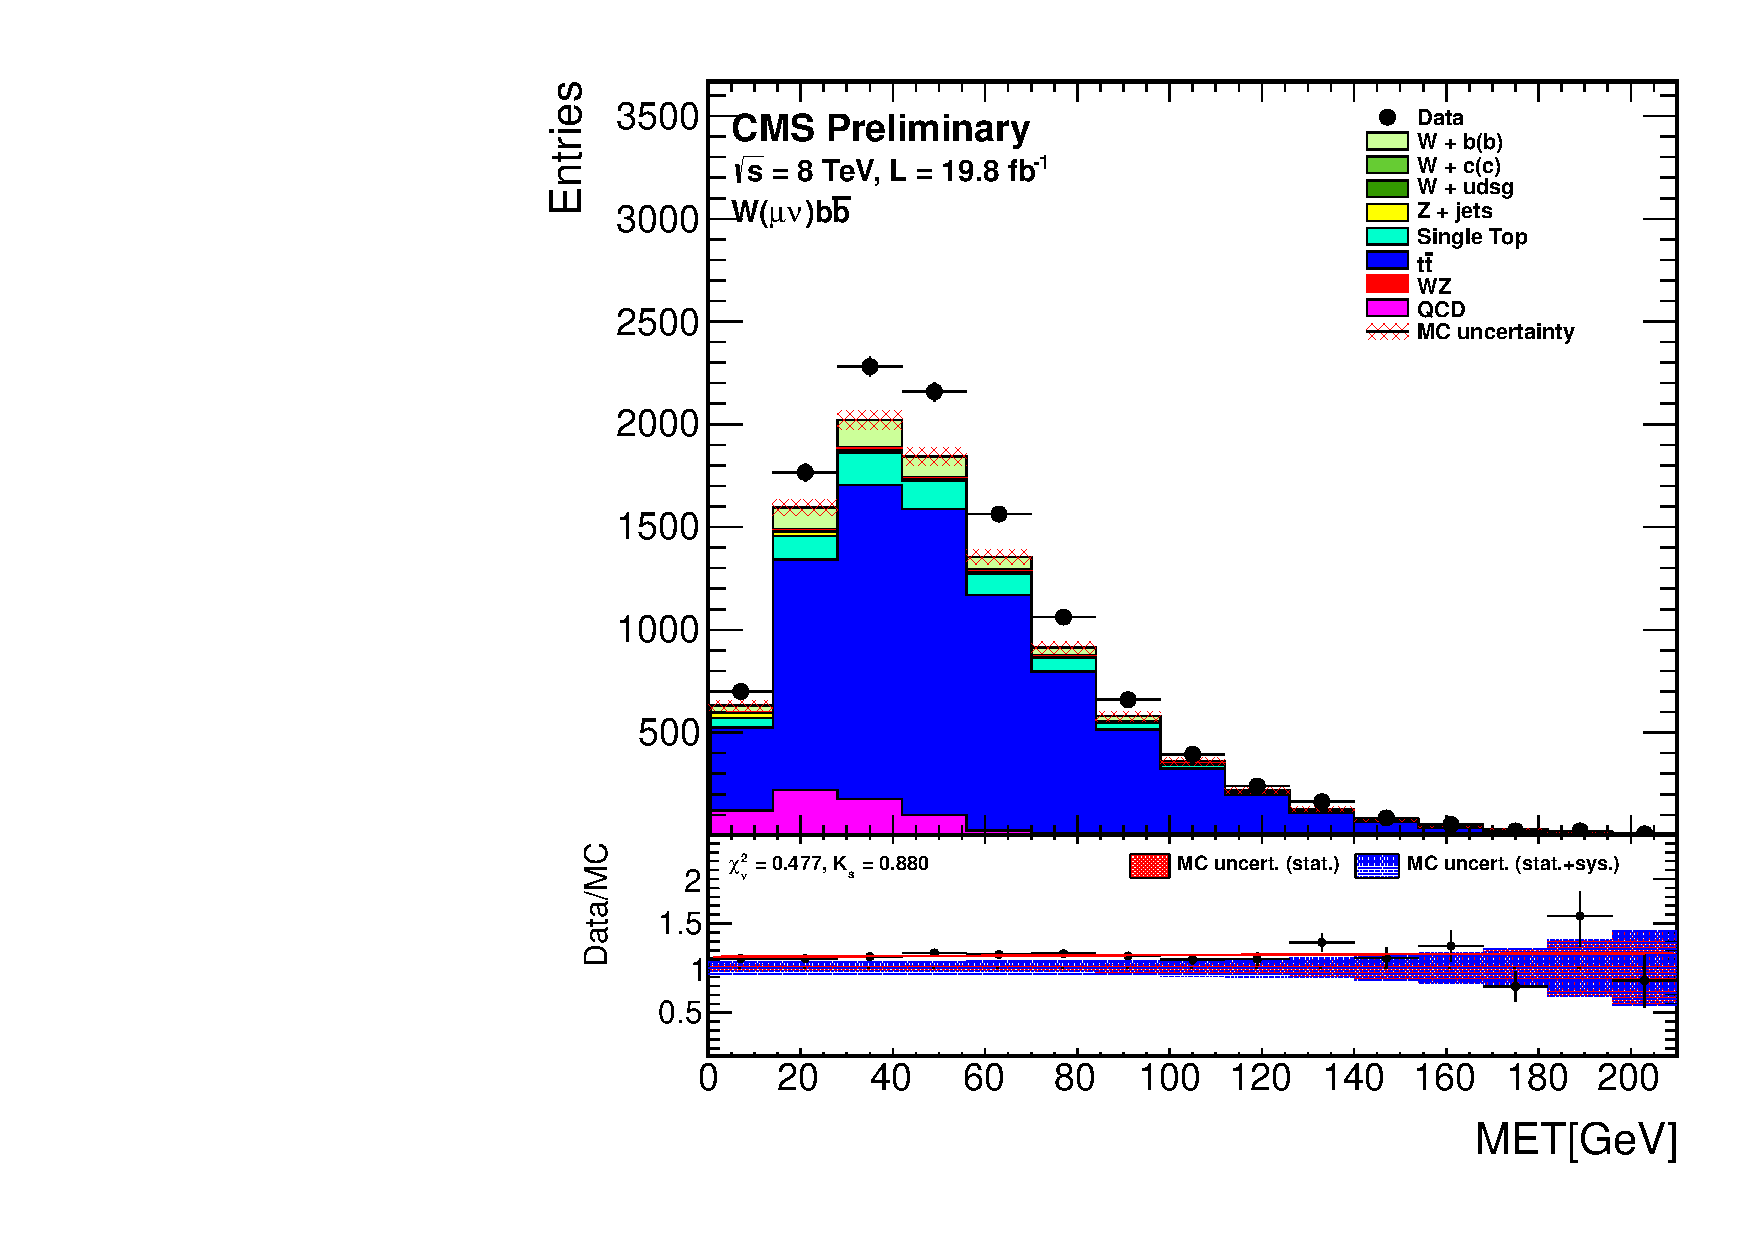
\includegraphics[width=0.48\textwidth]{Figures/Results/TT_GetMET_doQCD1.pdf}
		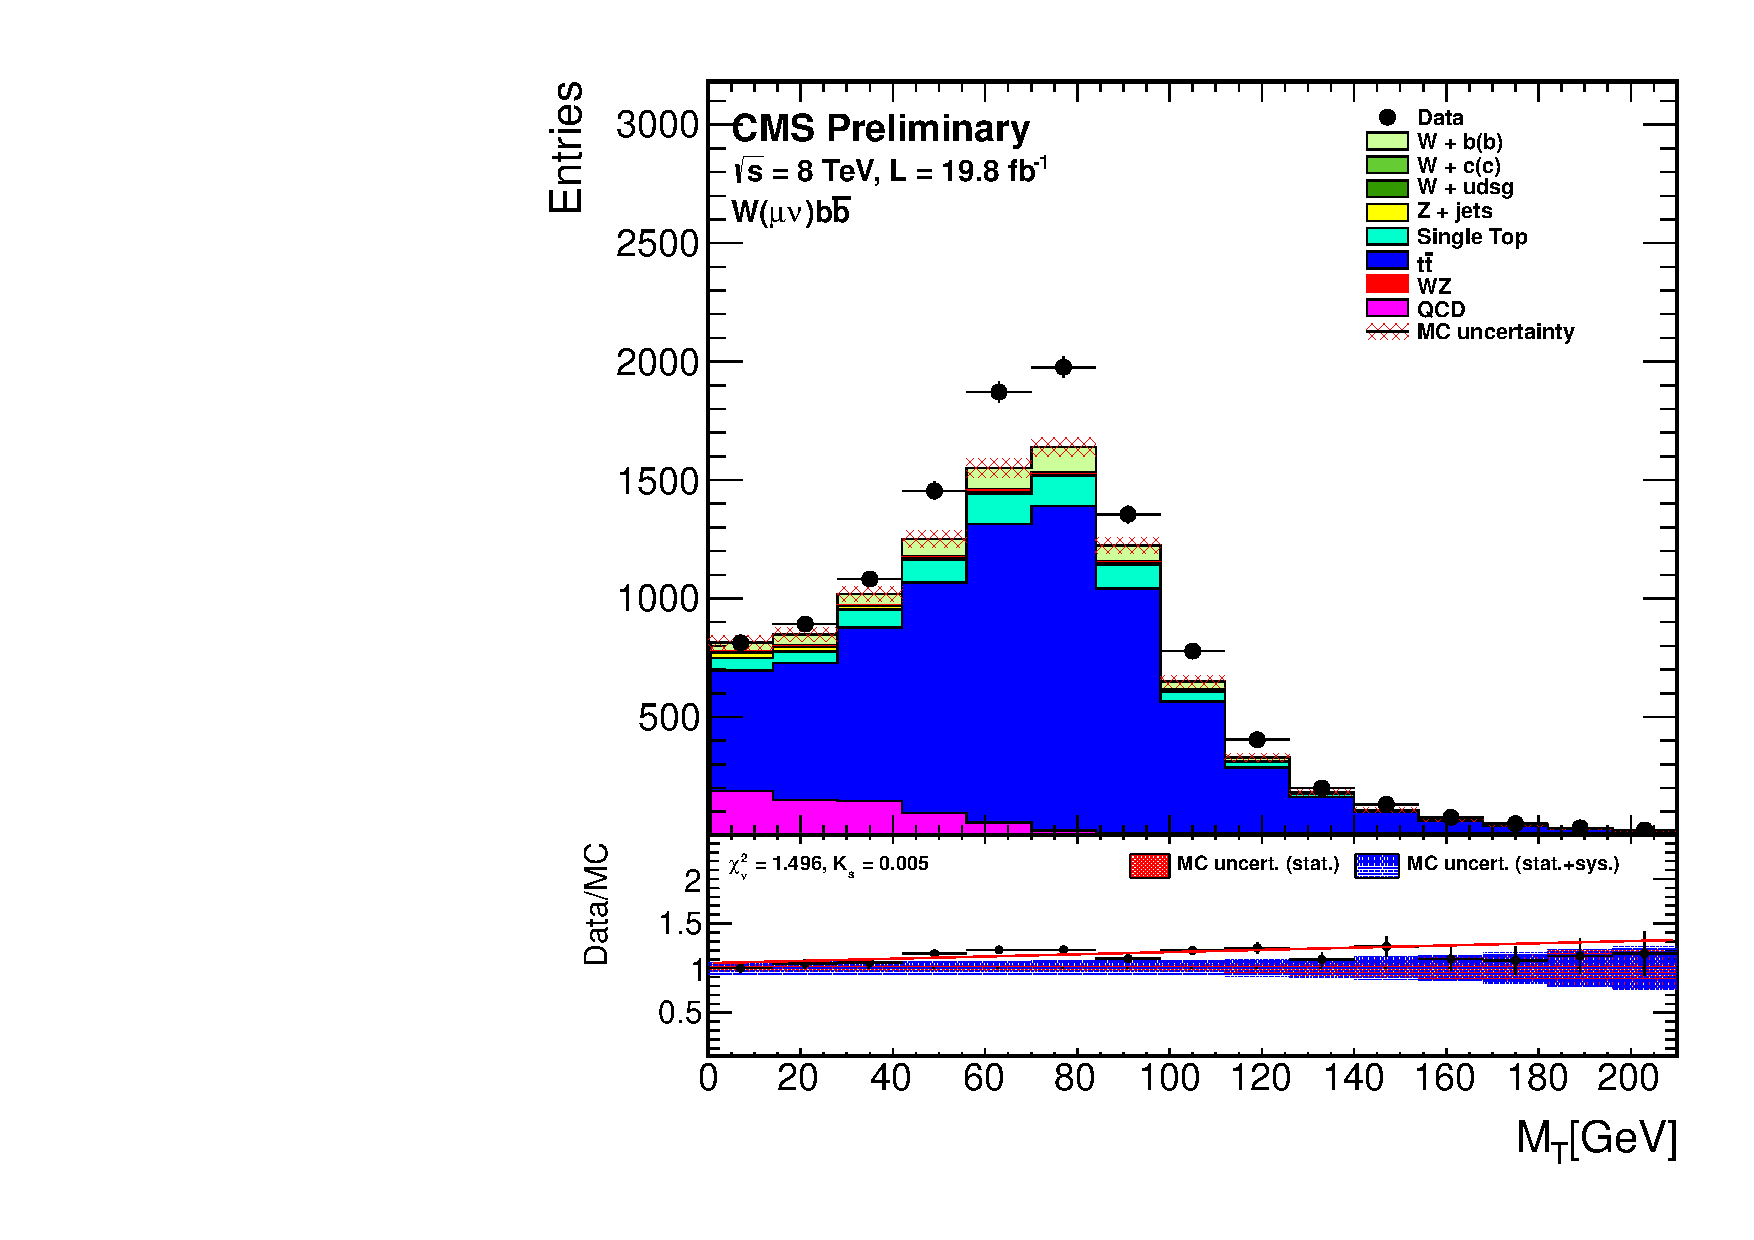
\includegraphics[width=0.48\textwidth]{Figures/Results/TT_GetVMt_doQCD1.pdf}
		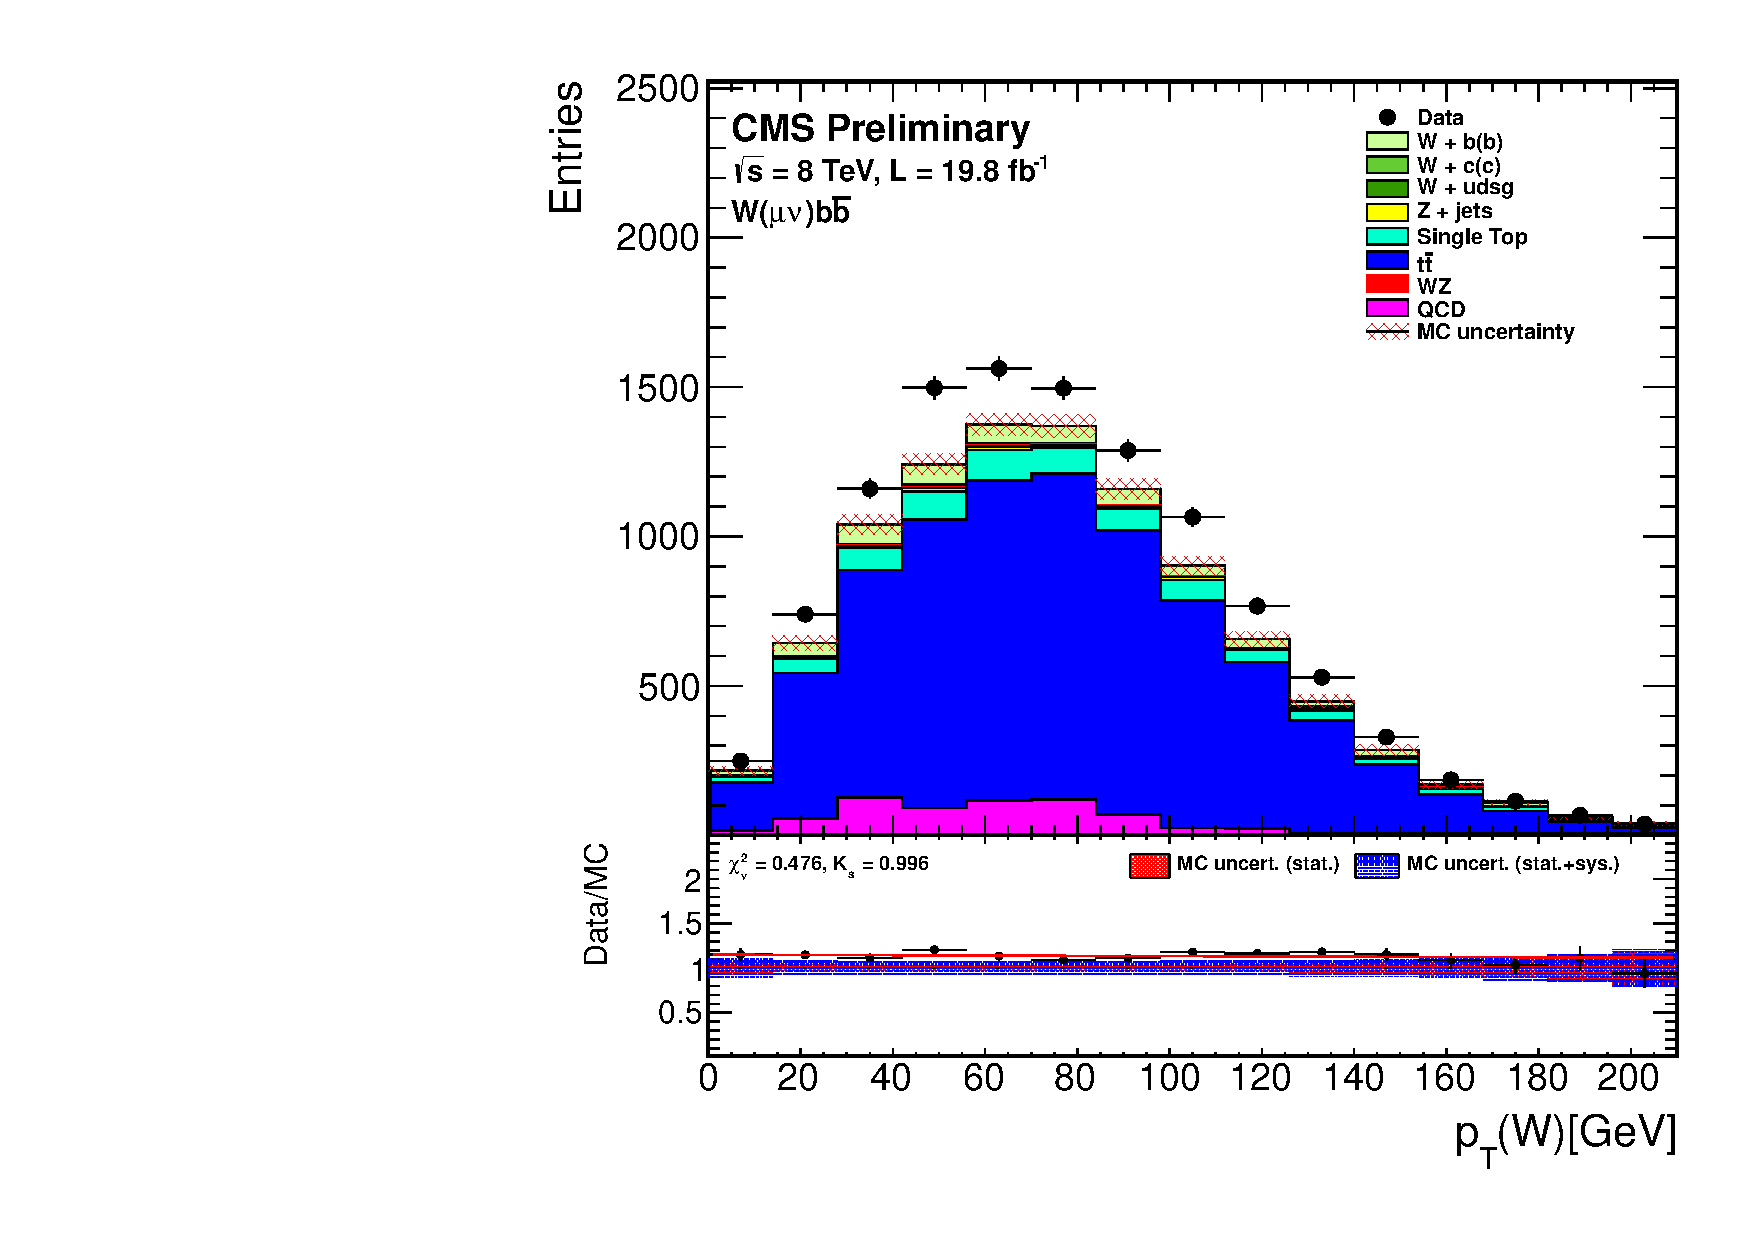
\includegraphics[width=0.48\textwidth]{Figures/Results/TT_GetWpt_doQCD1.pdf}
		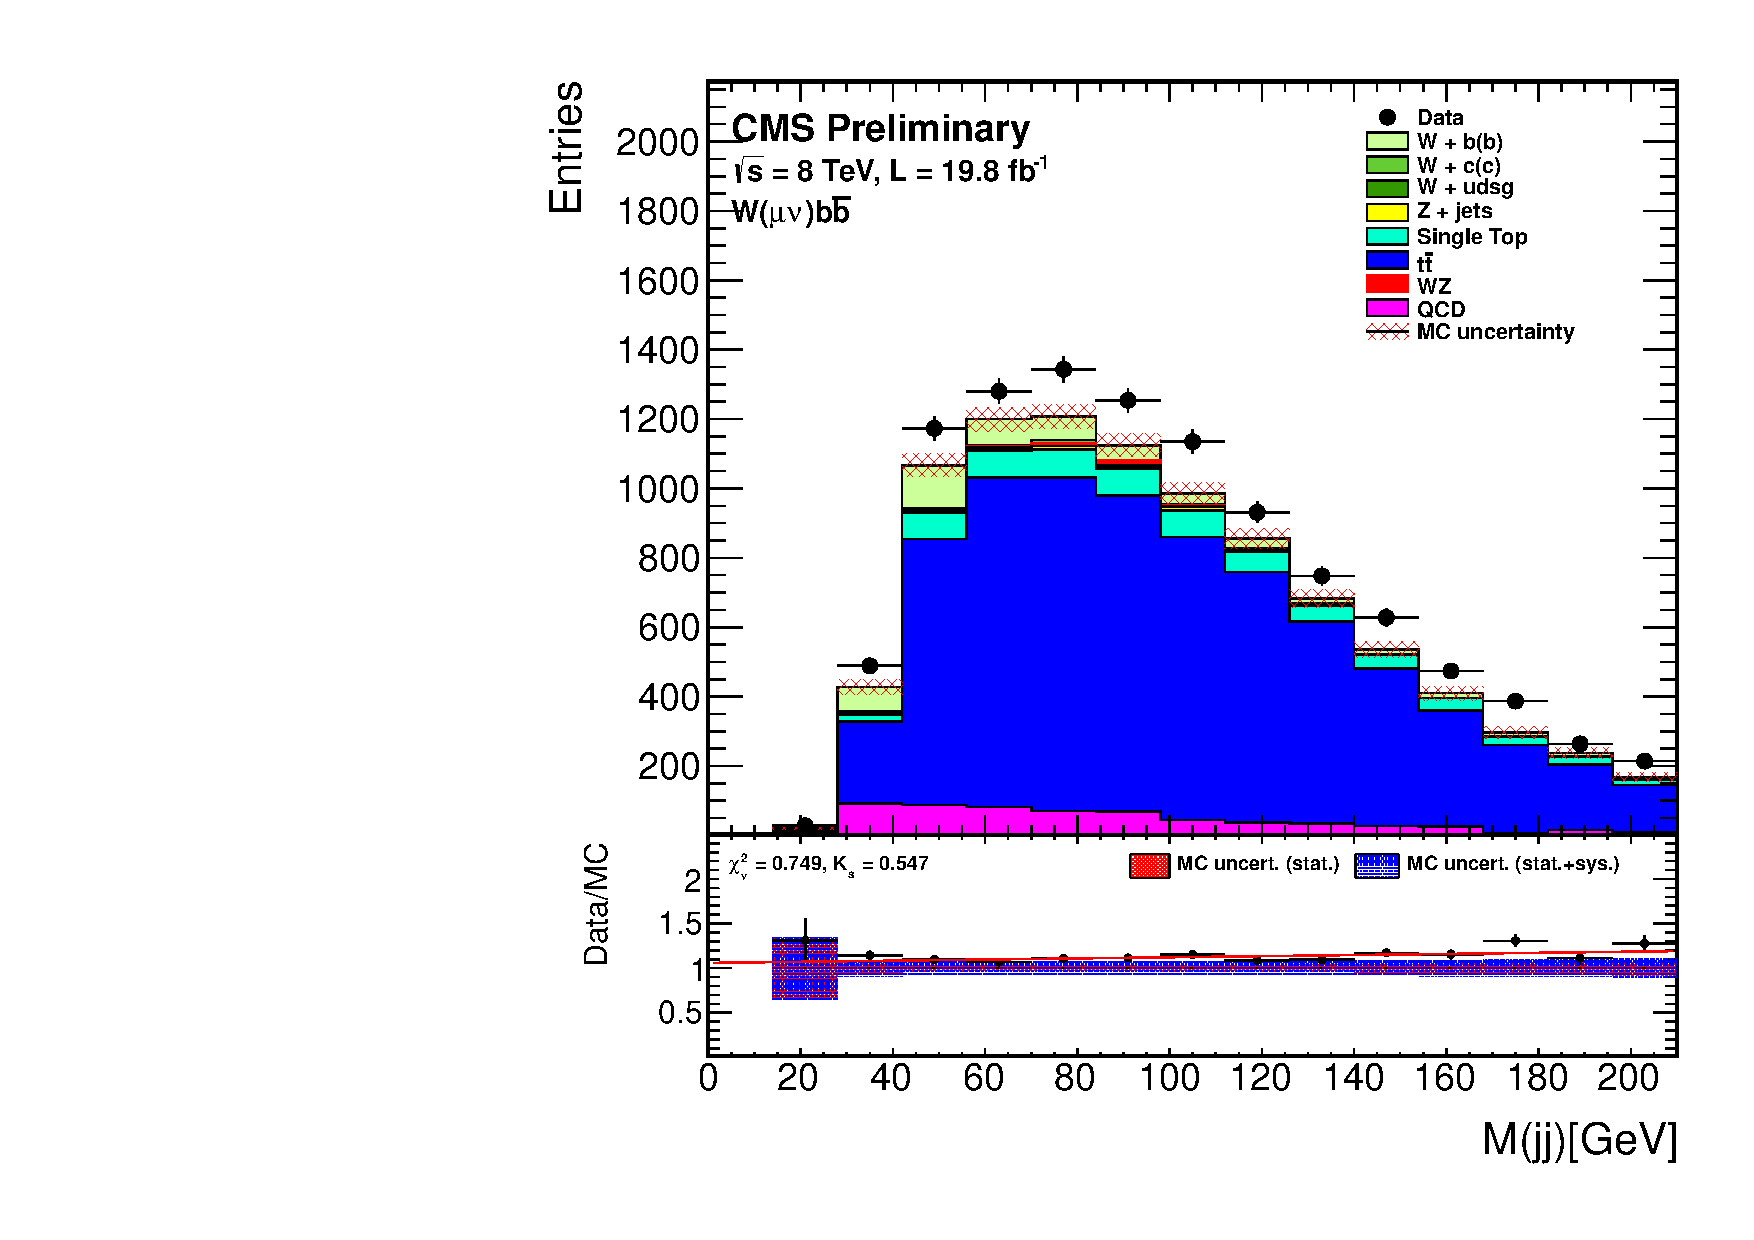
\includegraphics[width=0.48\textwidth]{Figures/Results/TT_H_mass_doQCD1.pdf}		
		%\rule{35em}{0.5pt}
	\caption[Top quark control region]{Top quark control region. Good shape agreement between data and simulation is observed, however simulation normalization is smaller than expected from data.}
	\label{fig:TT_CR}
\end{figure}

\subsection{Z+jets}

The contribution from the events where Z boson is produced in association with two b jets is largely suppressed by requiring only one lepton in the event. However, it can happen that one of the leptons from Z decay escapes the detection or is missidentified which possibly causes significant missing energy. Such events are than passing all selection criteria and have to be taken into account in the final cross section measurement. 

\subsection{W+light jets and W+charm}

W+jets is the major background before applying the b-tagging criteria which can be visible in figure \ref{fig:Wjets}. Both shape and normalization agree well between data and Monte Carlo for several distributions shown. Very tight b-tag selection reduces both W+light jets and W+charm to almost negligible levels.  

\begin{figure}[htbp]
	\centering
		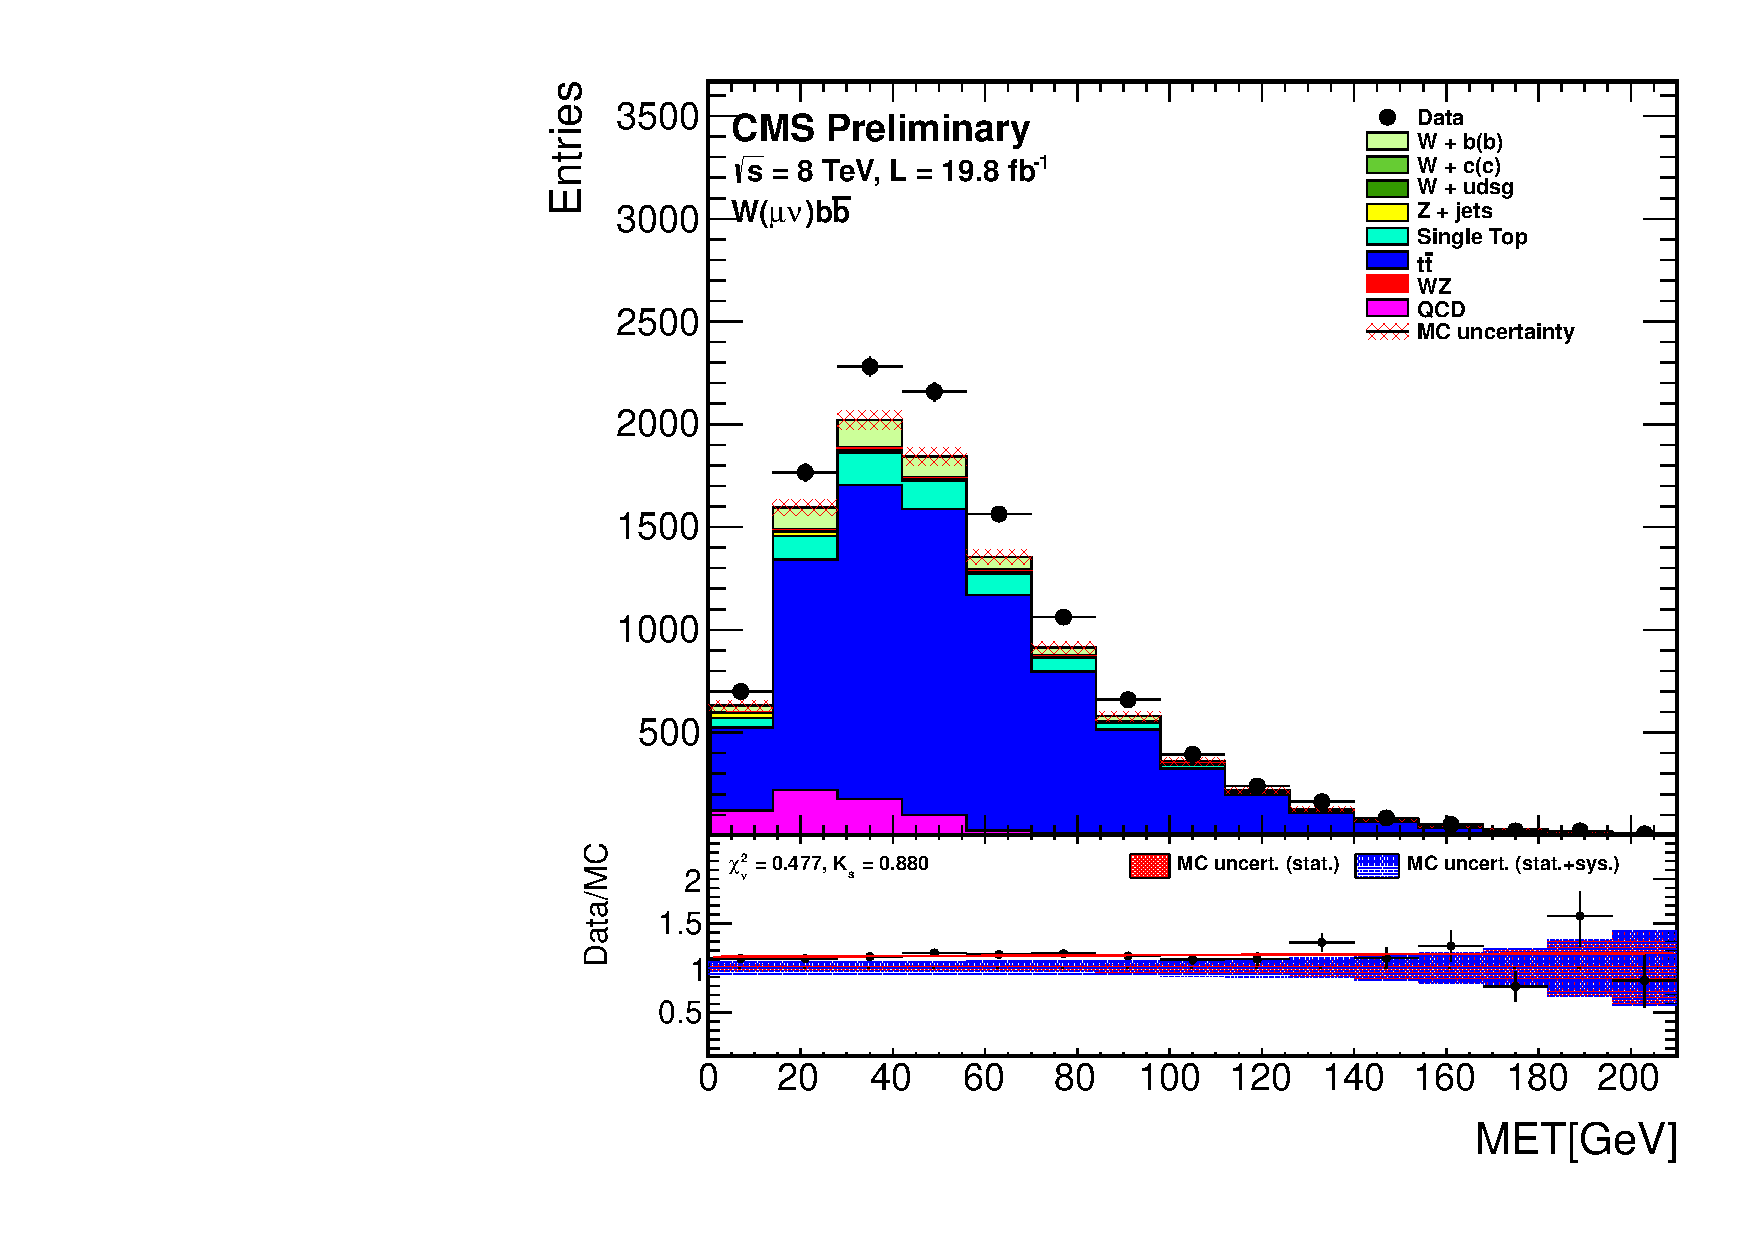
\includegraphics[width=0.48\textwidth]{Figures/Results/TT_GetMET_doQCD1.pdf}
		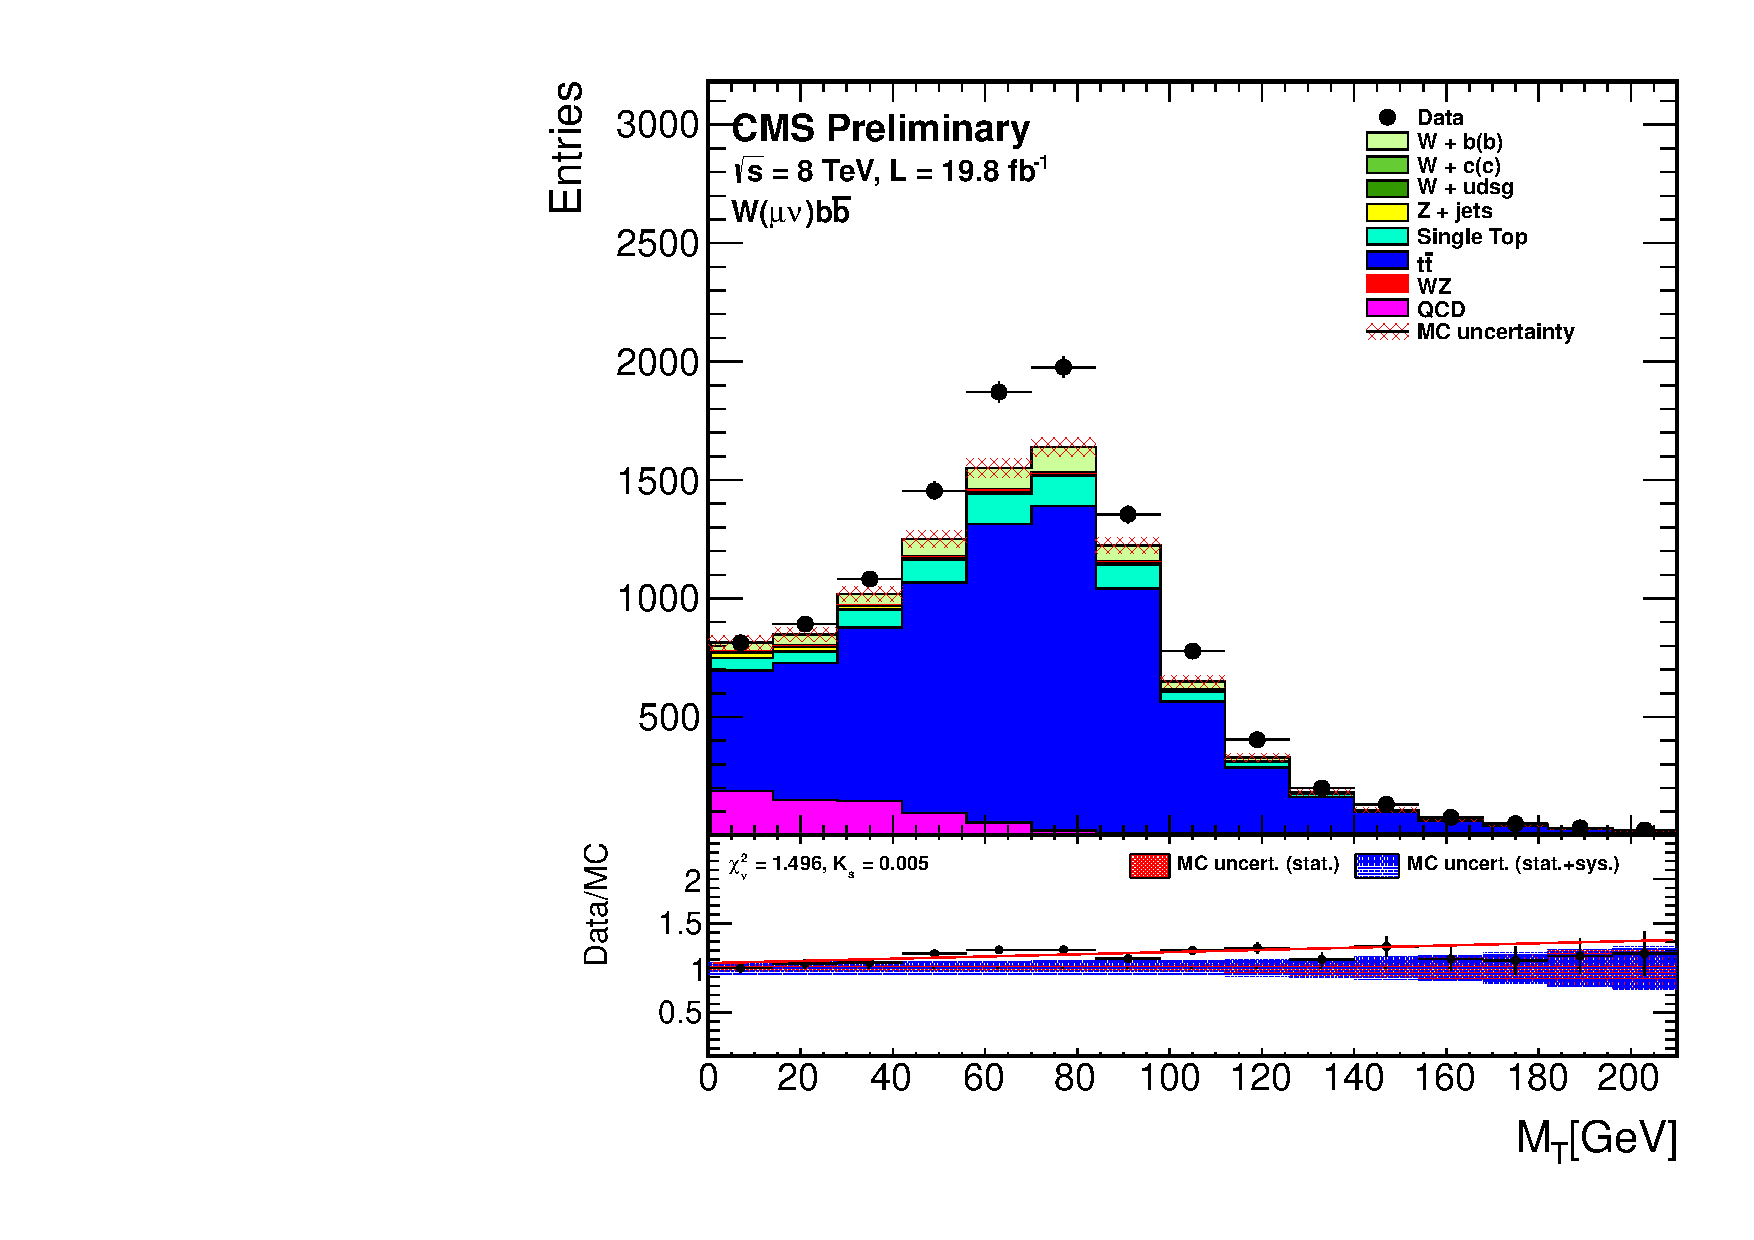
\includegraphics[width=0.48\textwidth]{Figures/Results/TT_GetVMt_doQCD1.pdf}
		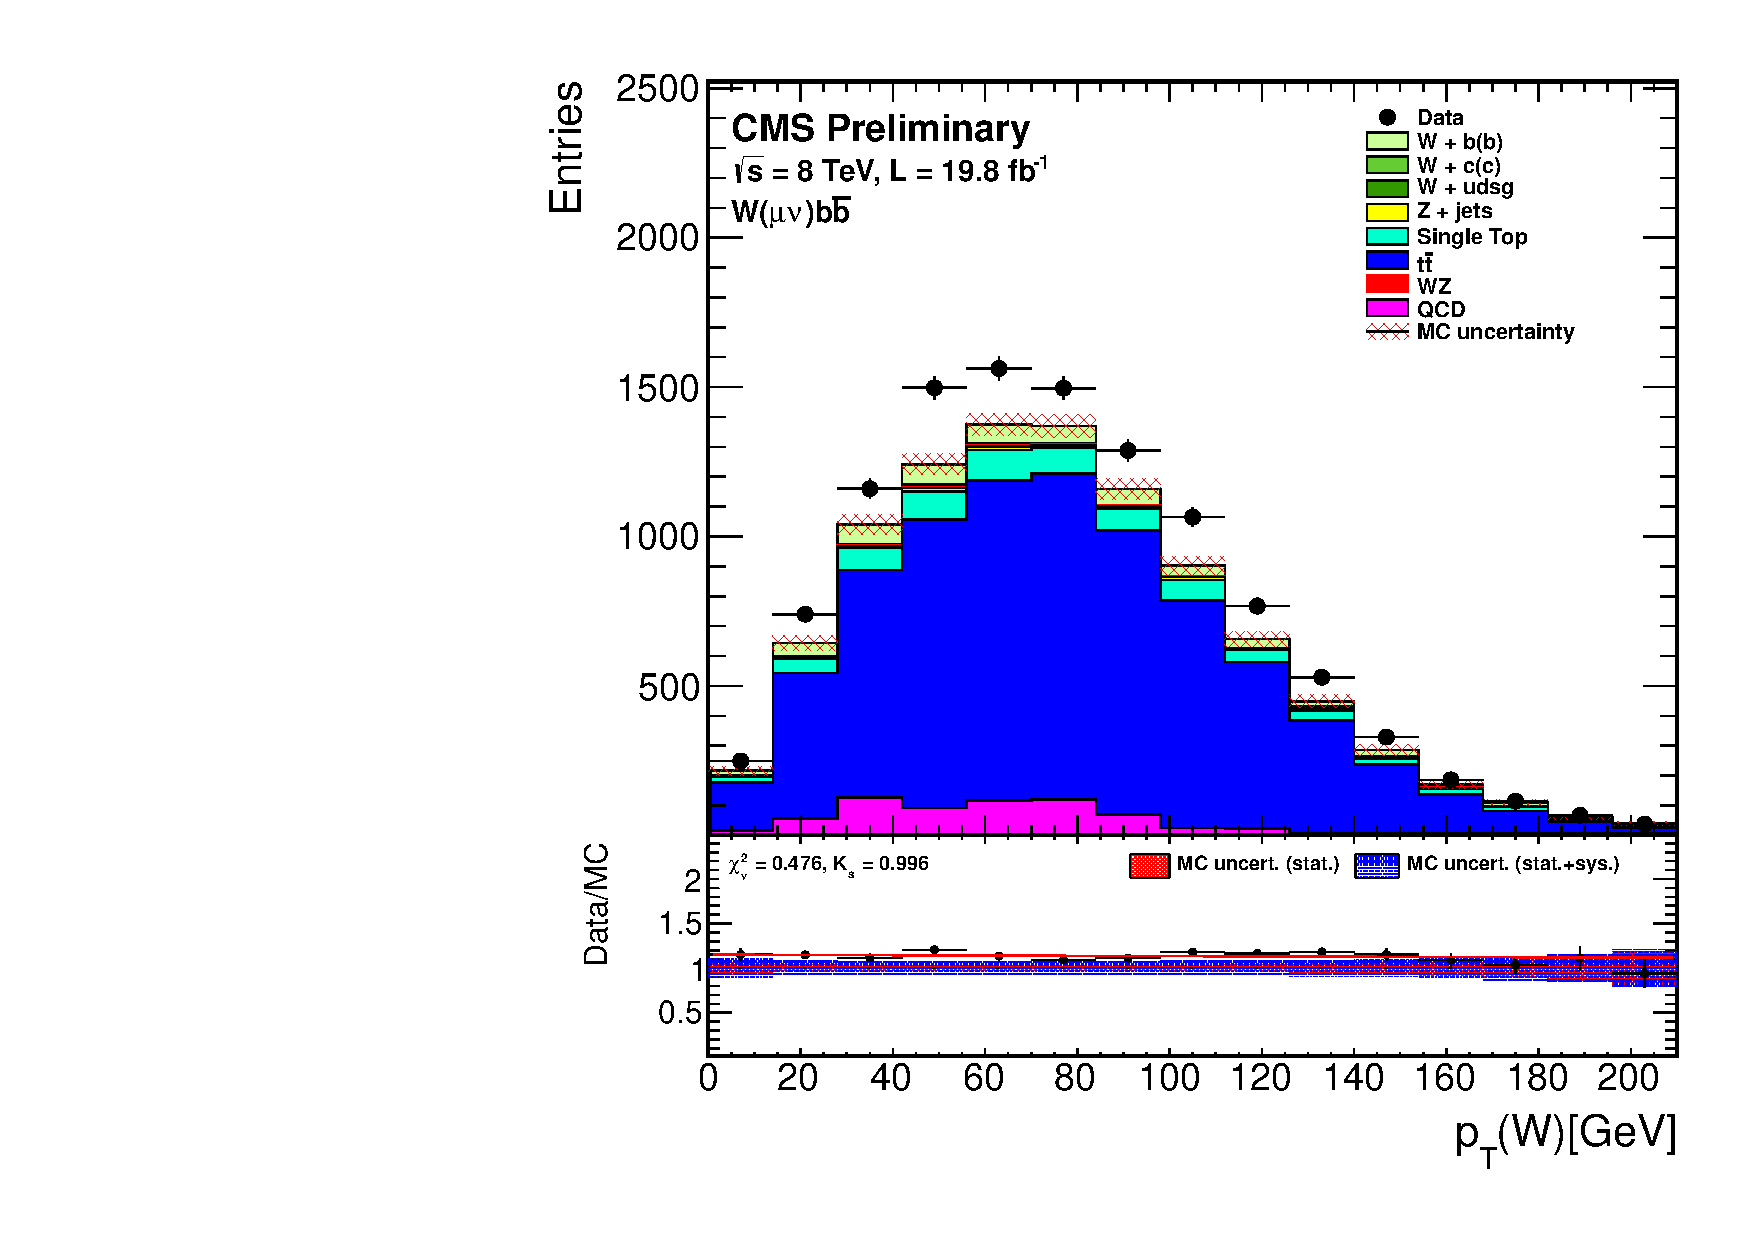
\includegraphics[width=0.48\textwidth]{Figures/Results/TT_GetWpt_doQCD1.pdf}
		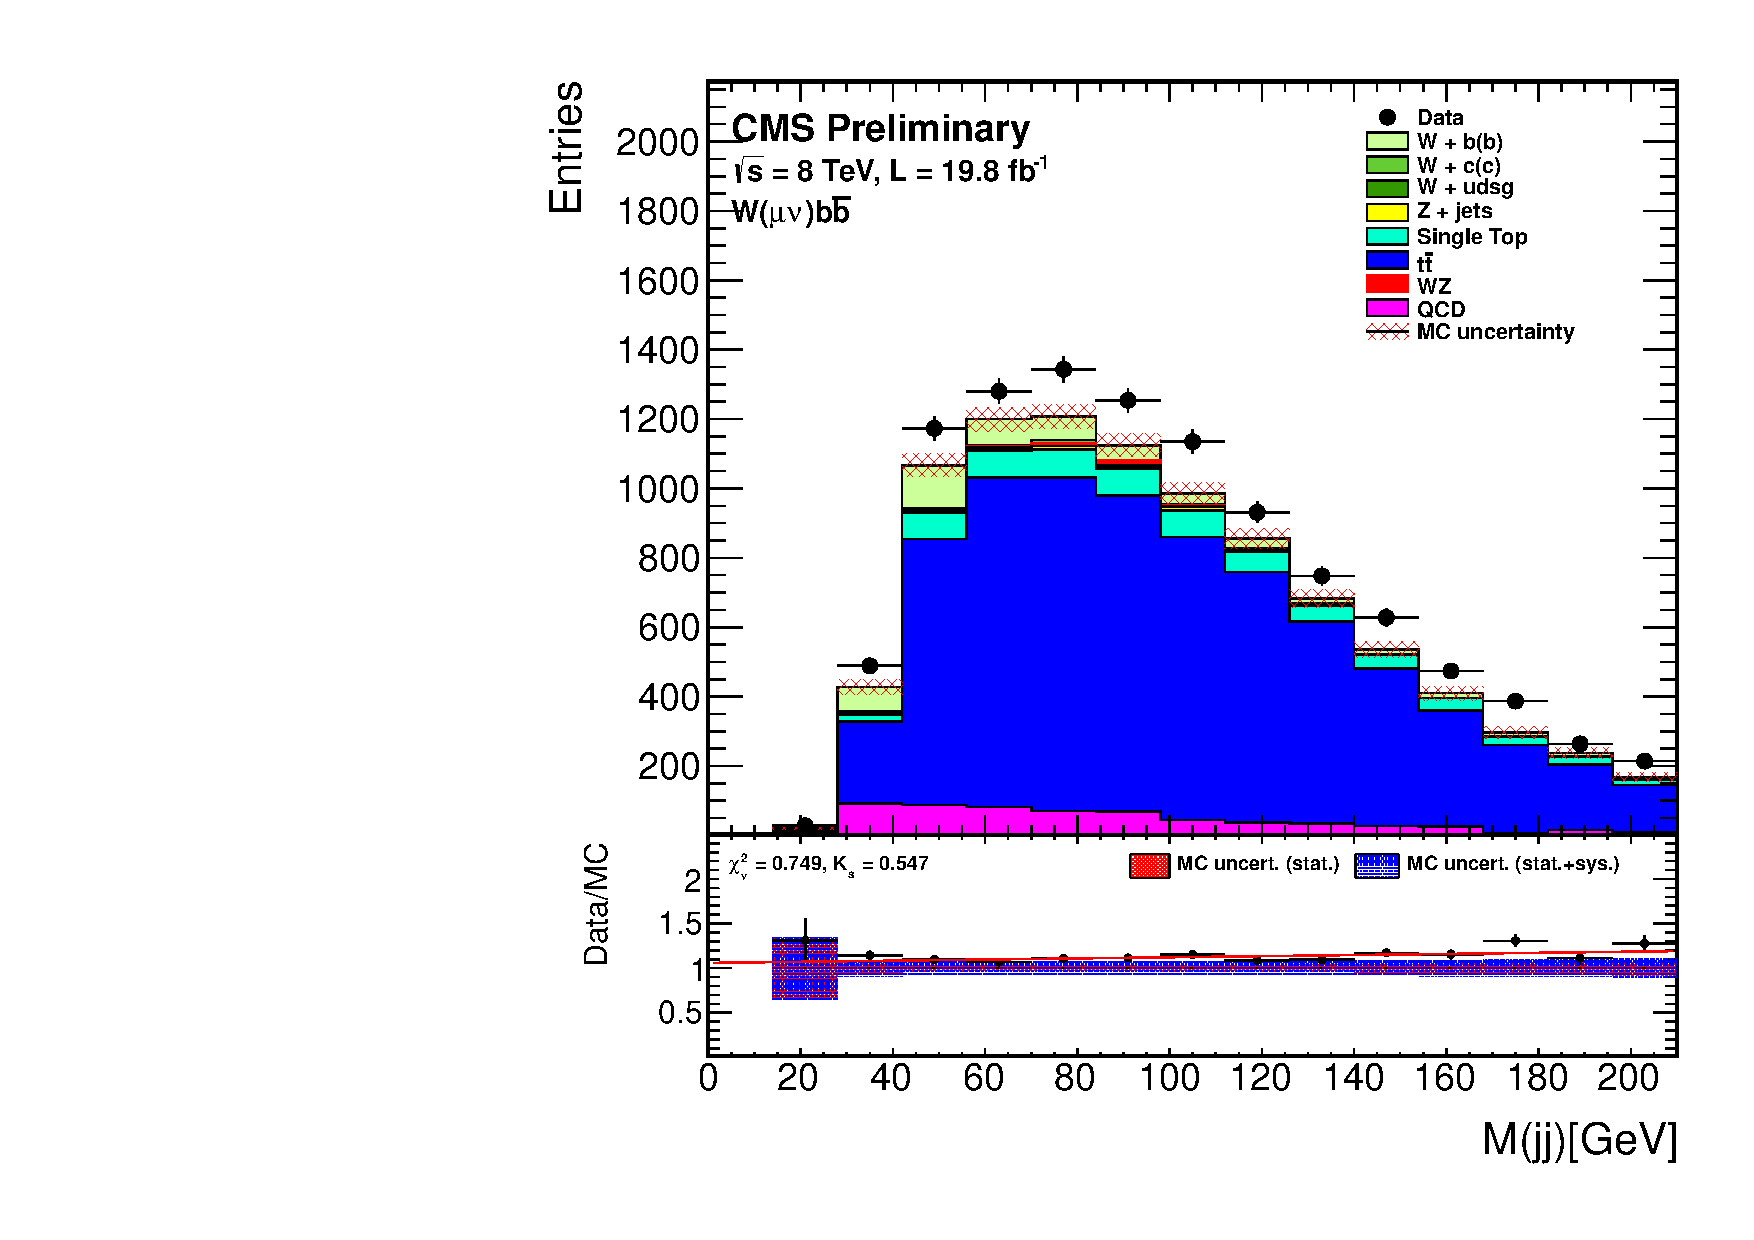
\includegraphics[width=0.48\textwidth]{Figures/Results/TT_H_mass_doQCD1.pdf}		
		%\rule{35em}{0.5pt}
	\caption[Distribution obtained using Wbb event selection before applying b-tagging criteria.]{Distribution obtained using Wbb event selection before applying b-tagging criteria.}
	\label{fig:Wjets}
\end{figure}

\subsection{QCD}

QCD background arises from QCD events containing soft leptons. An example of such event is shown in the left part of figure \ref{fig:QCD}. This is one of the more challenging backgrounds as it is difficult to simulate significant amount of such events without restrictions. Therefore, the contribution of QCD events in the signal region is determined from data. The illustration of the method is shown in the right part of figure \ref{fig:QCD}. Two uncorrelated variables are chosen, in this case transverse mass and lepton isolation. Signal region is shown in the region A. Control sample dominated by QCD events is created by inverting the lepton isolation cut to $iso>0.2$($0.15$) for muons(electrons) which is shown as region C. The rest of the selection criteria in the control sample is the same as in signal region. It is assumed that the QCD distribution has the same shape in regions A and C. The obtained sample is relatively clean, the shape of the distribution is determined by subtracting the simulation events that pass the selection. Normalization of the distribution is determined form the $M_T$ region below 30 GeV. Fake rate is determined from regions B and D by subtracting simulation number of simulated events that pass the cuts from the number of data events. The final normalization is than expressed as:
\begin{equation}
QCD^A=\frac{N^B_{data}-N^B_{MC}}{N^D_{data}-N^D_{MC}}\times QCD^{C}_{data}
\end{equation}       
where $N^B_{data}$ and $N^D_{data}$ are the number of data events in data in regions B and D respectively, and $N^C_{MC}$ and $N^D_{MC}$ are the number of MC events in regions B and D respectively. The signal region before and after the QCD contribution determination is shown in figure \ref{fig:QCD_dist}.
\begin{figure}[htbp]
	\centering
		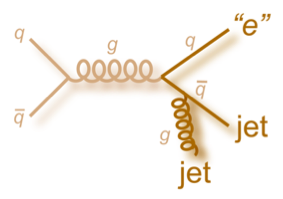
\includegraphics[width=0.4\textwidth]{Figures/QCD_diag.png}
		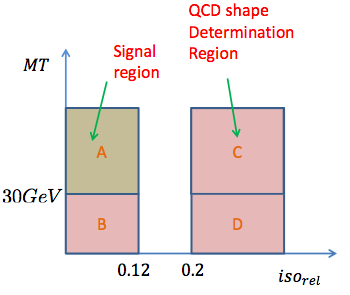
\includegraphics[width=0.45\textwidth]{Figures/QCD_AB.png}		
		%\rule{35em}{0.5pt}
	\caption[QCD diagram and illustration of QCD background determination]{An example of QCD event which looks like signal event (\textit{left}) and illustration of ABCD method used for QCD background determination(\textit{right})}
	\label{fig:QCD}
\end{figure} 

\begin{figure}[htbp]
	\centering
		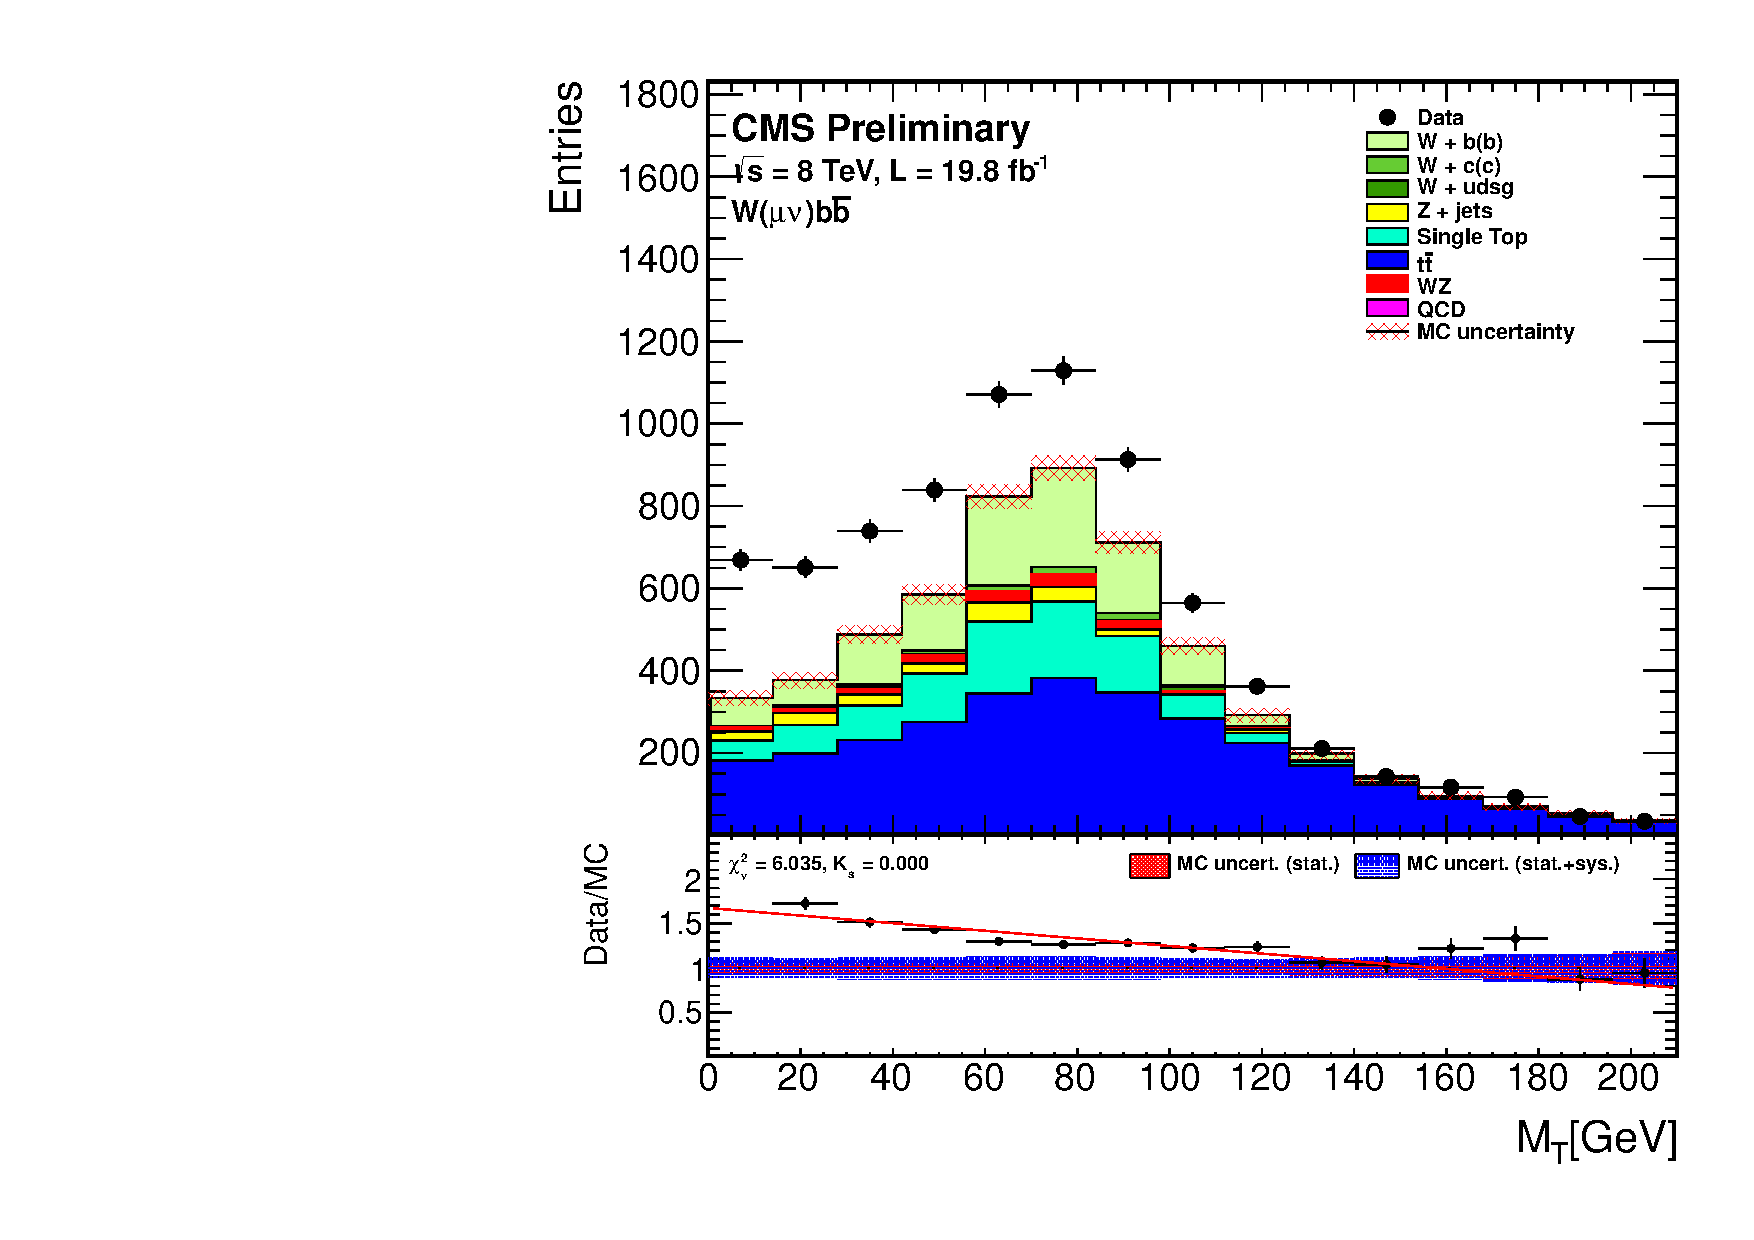
\includegraphics[width=0.48\textwidth]{Figures/VMt_QCD_before.pdf}
		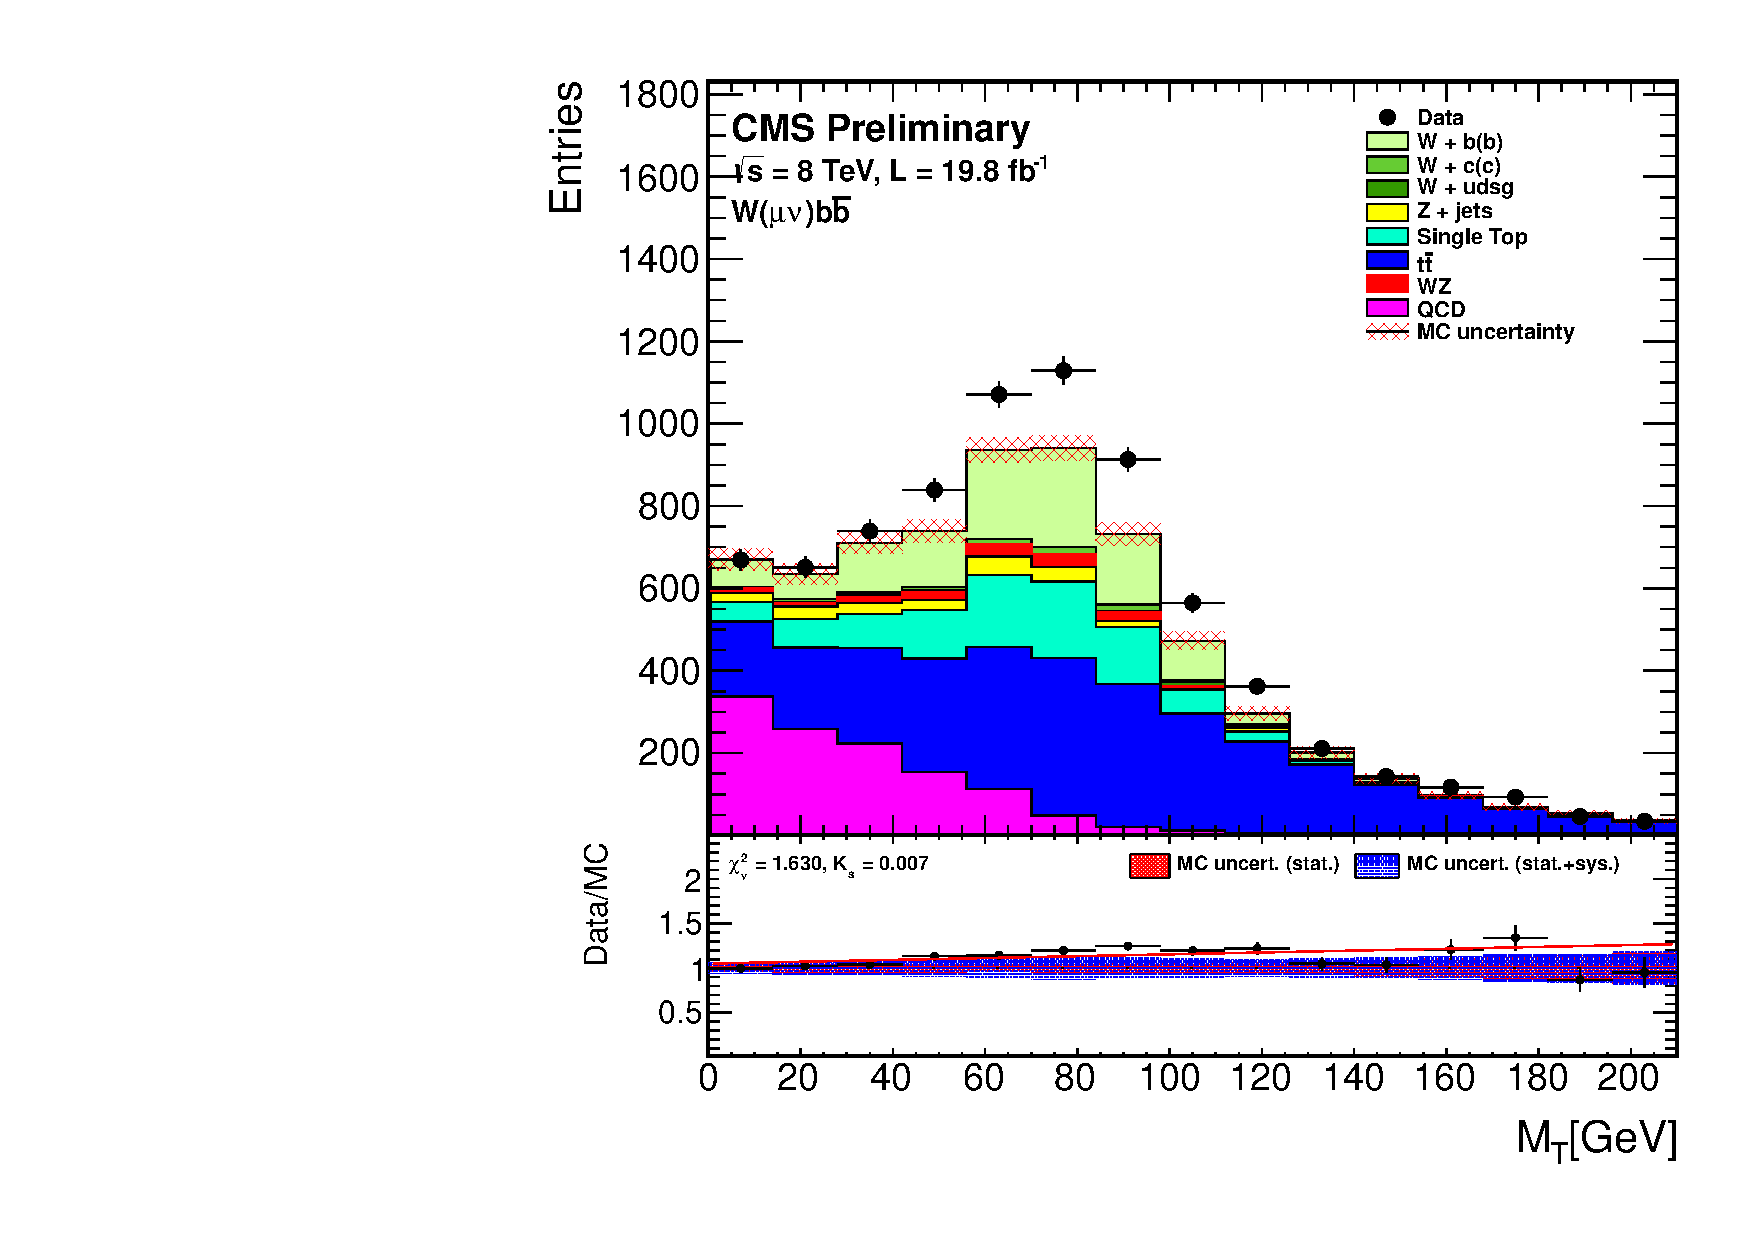
\includegraphics[width=0.48\textwidth]{Figures/VMt_QCD_after.pdf}		
		%\rule{35em}{0.5pt}
	\caption[Transverse mass distribution before and after QCD distribution determination.]{Transverse mass distribution before(\textit{left}) and after QCD background determination(\textit{right}).}
	\label{fig:QCD_dist}
\end{figure} 


\subsection{Other backgrounds}
Other backgrounds include processes with final states that match the final state of the signal. One of such signals is WZ where W decays leptonically and Z decays in a pair of b quarks. Another example is the production of Higgs boson in association with W boson where Higgs also decays to a pair of  quarks. Such backgrounds are called irreducible backgrounds.


%-----------------------------------
%	SECTION 3
%-----------------------------------
\section{Monte-Carlo corrections}
\label{sec:mcSF}

\subsection{Pileup}

In proton-proton collisions at high beam intensities, there is a high probability that multiple interactions could happen. These additional interactions are usually referred to as pileup interactions. The average number of additional interactions during 2012 was 21 with some events going up to 70. With these conditions it is important to be able to recognize the signature from such interactions. Usually pileup originates form low$-p_T$ QCD jets. The identification of pileup jets as well as their removal is described in detail in \cite{CMS:2013wea}. 
\par Simulated events have different distribution for number of pileup interaction with respect to data. This occurs because when generating simulated events, it was difficult to predict the exact pileup distribution in data. Therefore, simulated events to be rewighted to match the distribution in data. The data pile up distribution in the collision period was estimated assuming total proton-proton cross section of 68 mb. For each simulated event, a weight $w_{PU}$ is derived based on the number of pileup events provided by the generator. Figure \ref{fig:N_pu} shows number of pile-up events before and after the rewighting procedure for signal events in the muon channel. The agreement between data and simulation has clearly improved after the procedure. 

\begin{figure}[htbp]
	\centering
		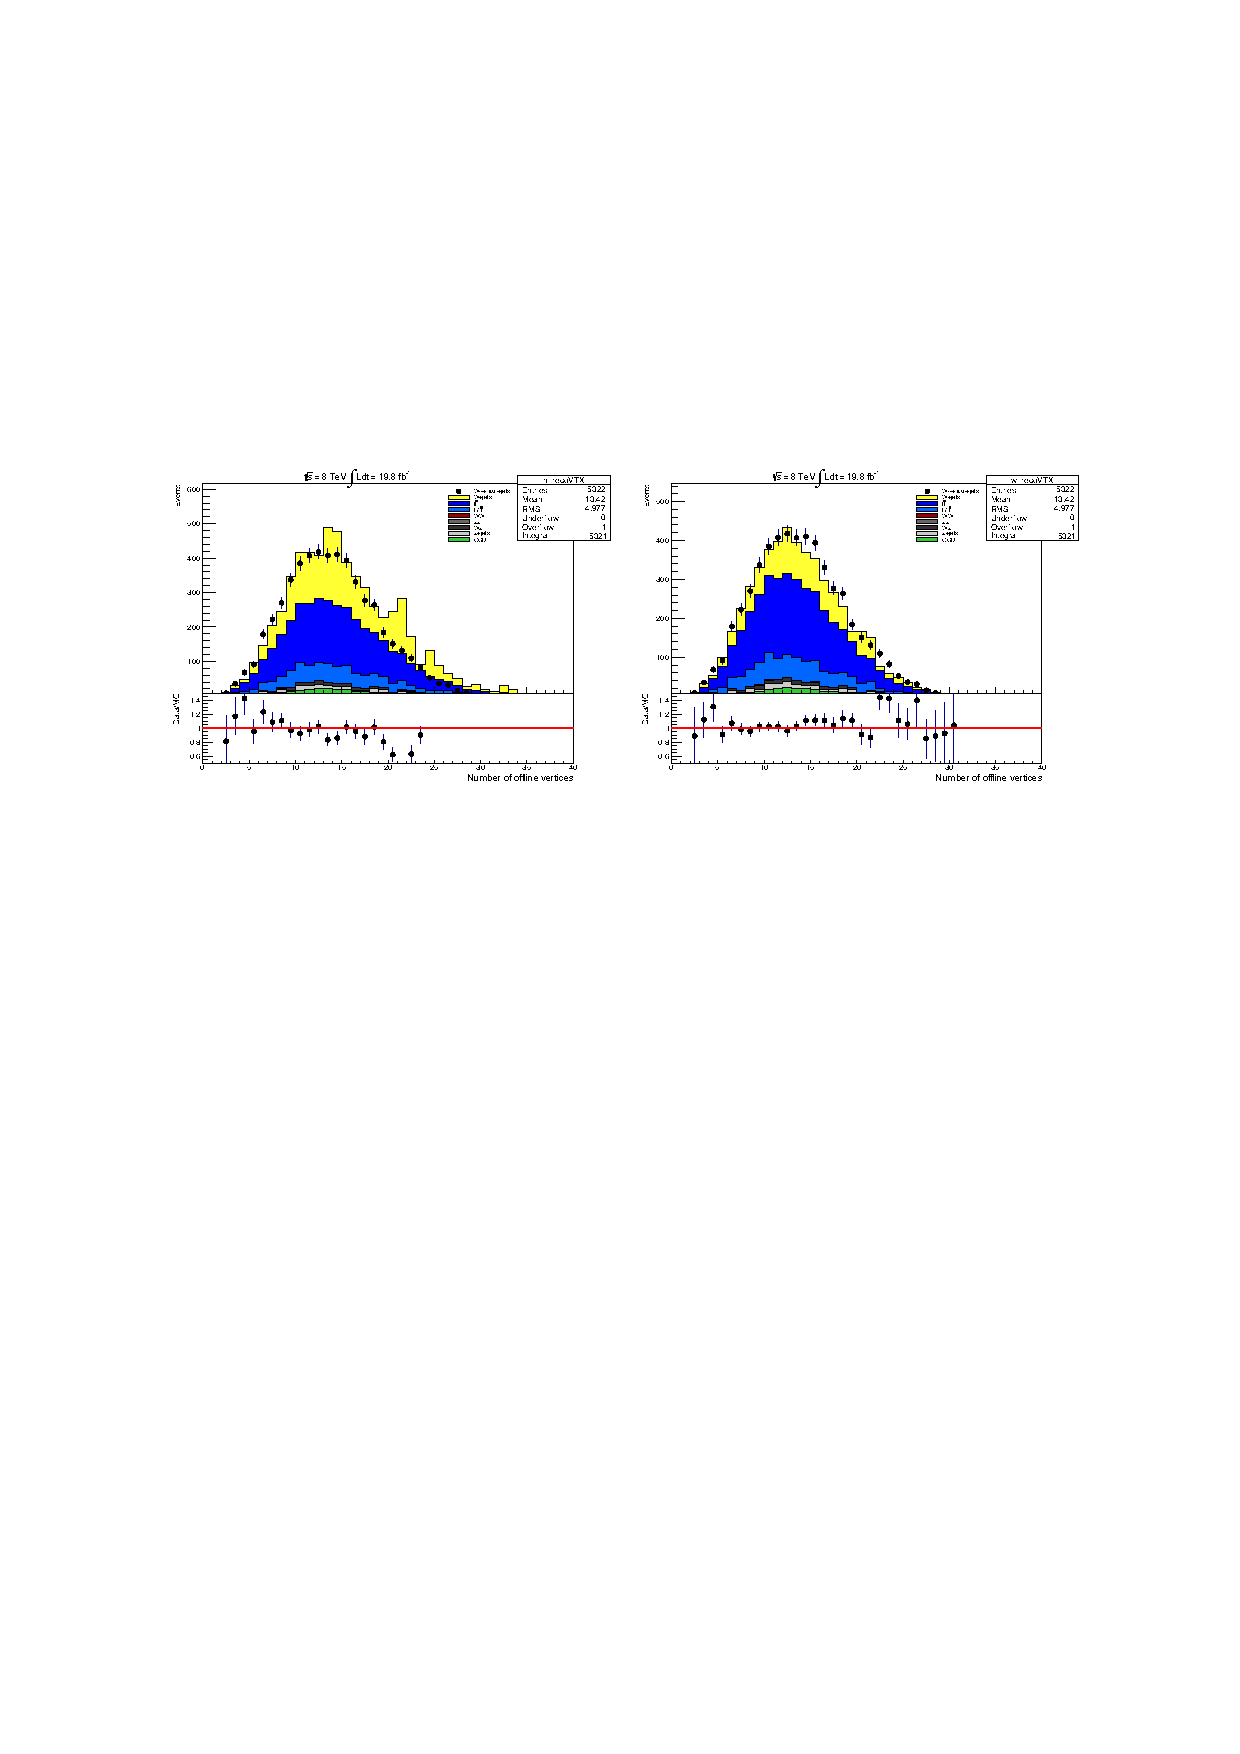
\includegraphics[width=0.9\textwidth]{Figures/NPU_placeholder.pdf}
		%\rule{35em}{0.5pt}
	\caption[Placeholder - PU]{Placeholder - $N_PU$}
	\label{fig:N_pu}
\end{figure} 

\subsection{Lepton efficiency measurement}

Events used for cross section measurement are required to pass certain triggers in order to be selected. However, trigger selection is not 100$\%$ efficient and the selection efficiency has to be measured. The following steps in the analysis like reconstruction and isolation have some inefficiencies as well. Efficiency estimation from simulation shows large systematic errors due to inaccuracy in signal modeling and detector response. This was the main motivation for development of the fully data-driven efficiency estimation called \textit{Tag and probe}. Using well-known mass resonances, such as Z boson mass resonance, a selection criteria is applied to the decay products. \textit{Tag} lepton is the one passing very tight selection cuts with low missidentification probability. The efficiency for certain cuts is than measured by counting \textit{probe} leptons which are leptons passing this looser cut divided by number of all leptons. Probes are selected in such way that the invariant mass of the two leptons falls into the Z mass resonance. The following relation is used for the measurement:
\begin{equation}
\epsilon = \frac{N_{pass}}{N_{pass}+N_{fail}}
\end{equation}   
Final selection contains a number of events where Z boson was not actually produced and which have to be subtracted. Both signal and background contributions are parametrized their relative contributions are estimated using Maximum likelihood fit. For signal events a convolution of Z generator shape with a Gaussian is used to take into account the detector effects, while for background parametrization, a combination of exponential function and polinomial was used.
\par The efficiency was measured as a function of pseudorapidity and transverse momentum of a passing probe. Trigger, identification and isolation criteria were used in electron and muon channels separately. Both data and Monte Carlo efficiencies were measured and their ratio was used as a scale factor for each event in order to match simulated lepton efficiencies to measured data. Muon identification and isolation efficiency measurement for data and MC is shown in figure \ref{fig:eff_IDISO} while trigger efficiency measurement is shown in figure \ref{fig:eff_trig}.

\begin{figure}[htbp]
	\centering
		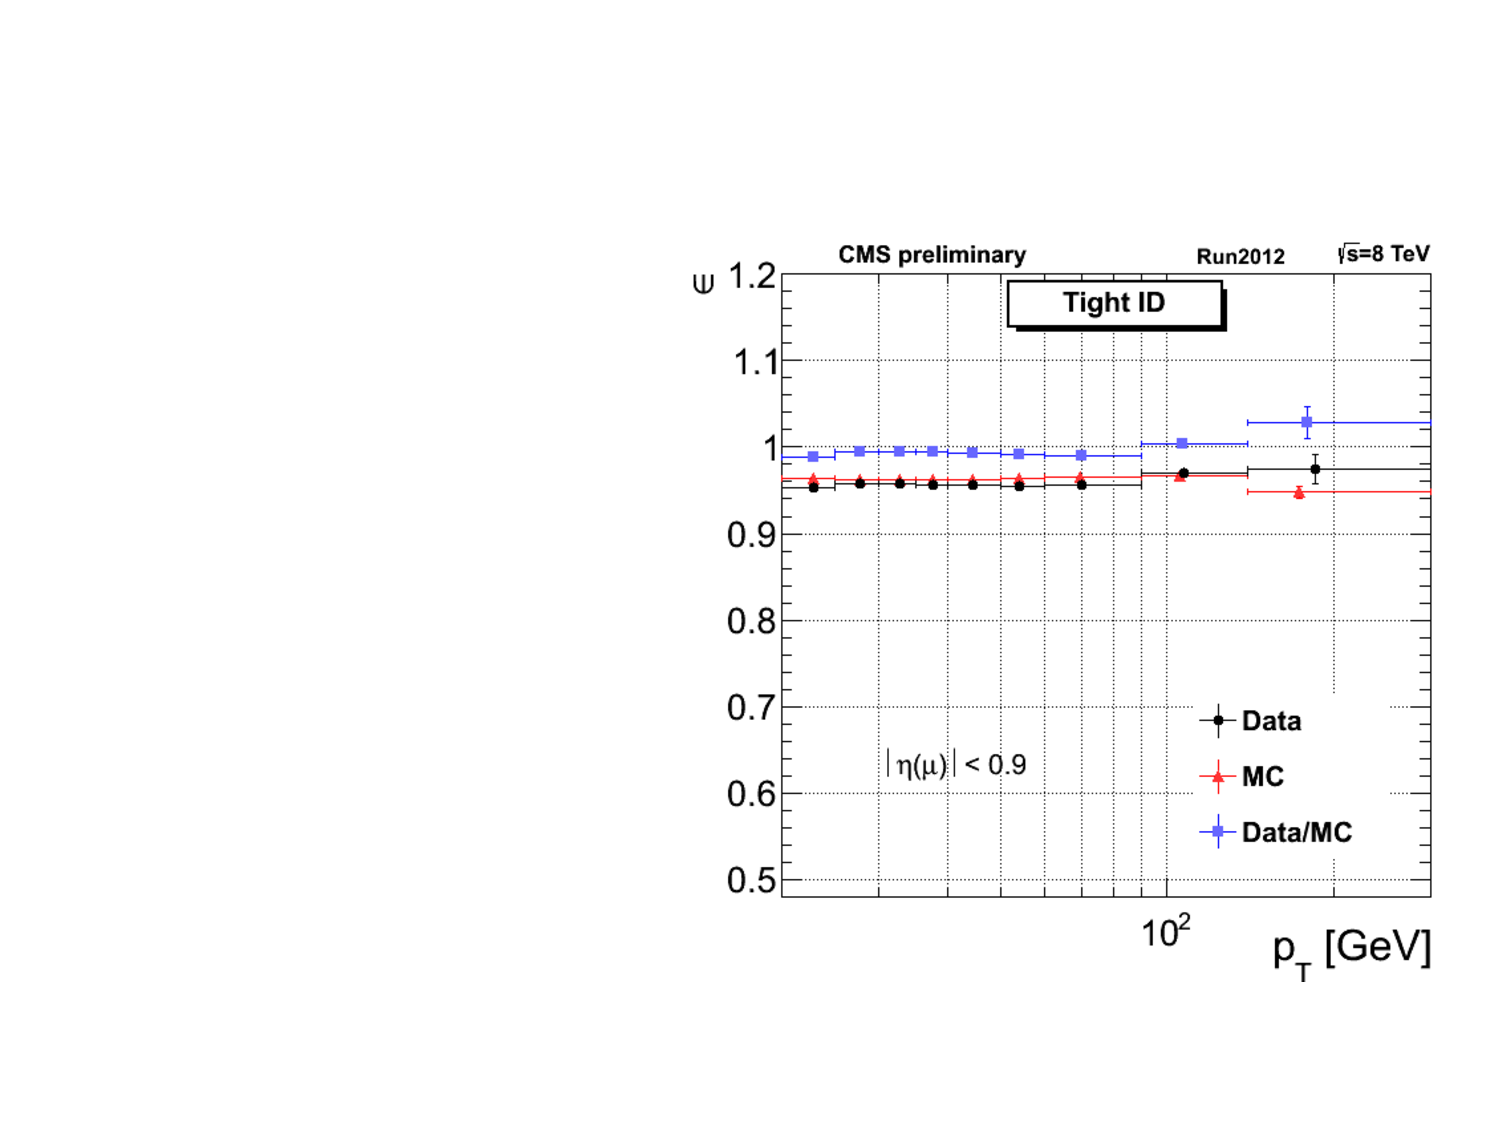
\includegraphics[width=0.49\textwidth]{Figures/ID_eff.pdf}
		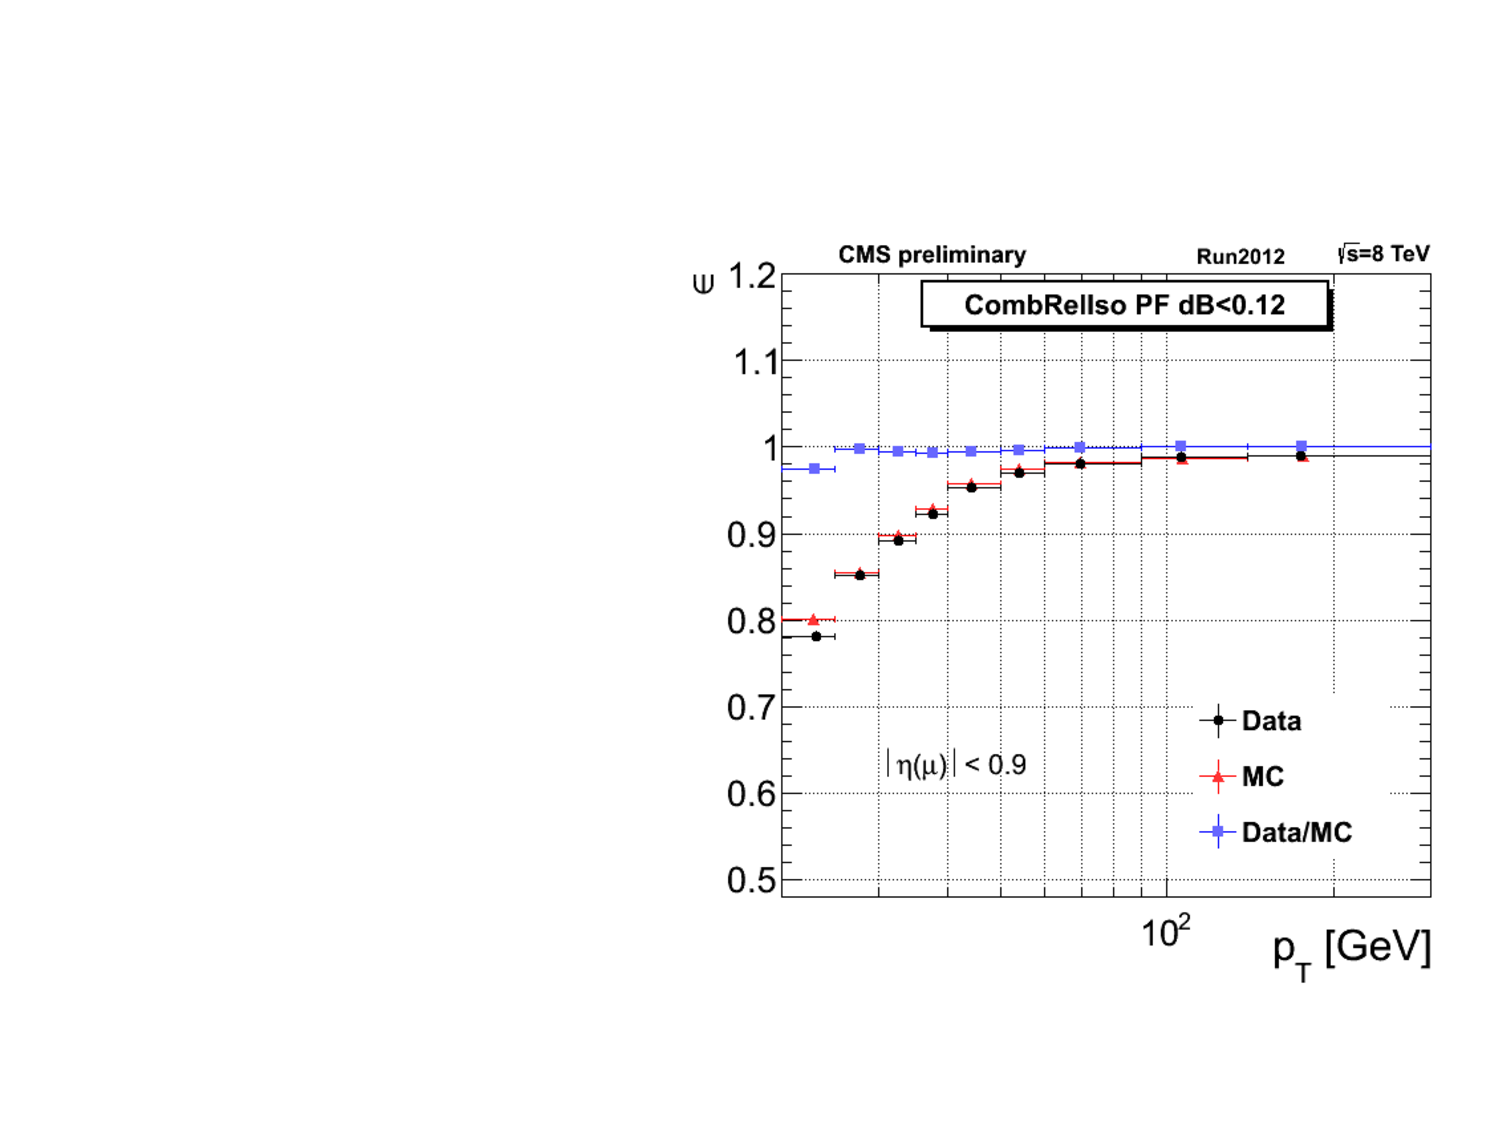
\includegraphics[width=0.49\textwidth]{Figures/ISO_eff.pdf}
		%\rule{35em}{0.5pt}
	\caption[Muon identification and isolation efficiencies using \textit{tag and probe} method.]{Muon identification and isolation efficiencies as a function of a probe $p_T$ using \textit{tag and probe} method. The measurement shown here is for barrel part of the detector$(\eta<0.9)$, but similar measurements were performed for the region between barrel and endcap$(0.9<\eta<1.2)$ and endcap $(1.2<\eta<2.1)$ separately.}
	\label{fig:eff_IDISO}
\end{figure}

\begin{figure}[htbp]
	\centering
		\includegraphics[width=0.5\textwidth]{Figures/trig_eff.pdf}
		%\rule{35em}{0.5pt}
	\caption[Muon trigger efficiency using \textit{tag and probe} method.]{Muon trigger efficiency for $\mathrm{HLT\_IsoMu24}$ using \textit{tag and probe} method of barrel part of the detector $(\eta<0.9)$.}
	\label{fig:eff_trig}
\end{figure}  



\subsection{\textit{b-tagging} scale factors}

CMS simulations describe very well the detector performance, however, it can be difficult to accurately model all parameters used in b-tagging algorithms. Procedure used to identify b-jets is described in \ref{sec:btagging} and it depends on track reconstruction efficiency, tracking resolution and other tracking related parameters. Efficiency and missidentification probability are functions of transverse momentum and pseudorapidity of a jet. Therefore, it is very important to determine the b-tagging efficiency from data. The obtained corrections are applied to simulated events as scale factors which is ratio between efficiency measured in collisions $\epsilon_b^{data}$ and efficiency from simulated events $\epsilon_b^{MC}$:
\begin{equation}
SF_b=\frac{\epsilon_B^{data}}{\epsilon_b^{MC}}
\end{equation}
Scale factor determination has to be performed using b-jet enriched sample such as $t\bar{t}$ or multijets events with jet containing a muon within a $\Delta R <0.4$ cone from the jet axis. The choice of the muon within jet relies on the fact that in B hadron decays, the semileptonic branching ratio is much higher that that for other hadrons ($\sim$ 20$\%$ when including c$\rightarrow$ decays) and such jets are much more likely to arise from B hadron decay. With very high muon detection efficiency at CMS, it is relatively easy to obtain a clean sample with jets containing nonisolated muons. Additional kinematic criteria is applied to the selected muons to determine the efficiency in different $p_T$ ranges of the jets. Other efficiency measurement is performed using $t\bar{t}$ enriched sample by cutting on number of selected jets and isolated leptons in the event and approximating that the $t$ quark decays to $W+b$ exclusively. By combining the results from both measurements, scale factors were obtained as a function of jet $p_T$ together with statistical and systematic error for each $p_T$ bin. The same strategy is used to obtain missidentification rates by using the inverted cut on b-tag discriminator. The behavior of both scale factors is approximated by an analytical parametrization as a function of jet $p_T$.  
The usage of the scale factors depends on the number of b-tagged jets in the event. In this analysis two b-tagged jets are required and weight for each event is derived as:
\begin{equation}
w(2|2)=SF_{b||light}(\mathrm{1st\ jet})\times SF_{b||light}(\mathrm{second\ jet})
\end{equation}
where $w(2|2)$ is event weight with 2 jets where both jets are b-tagged. The choice between $SF_{b}$ and $SF_{light}$ depends on the flavor of the jet in the simulation. A jet is considered a b jet if there is a B hadron present among the jet constituents within a cone of 0.4 from the jet axis.    

\begin{figure}
\centering
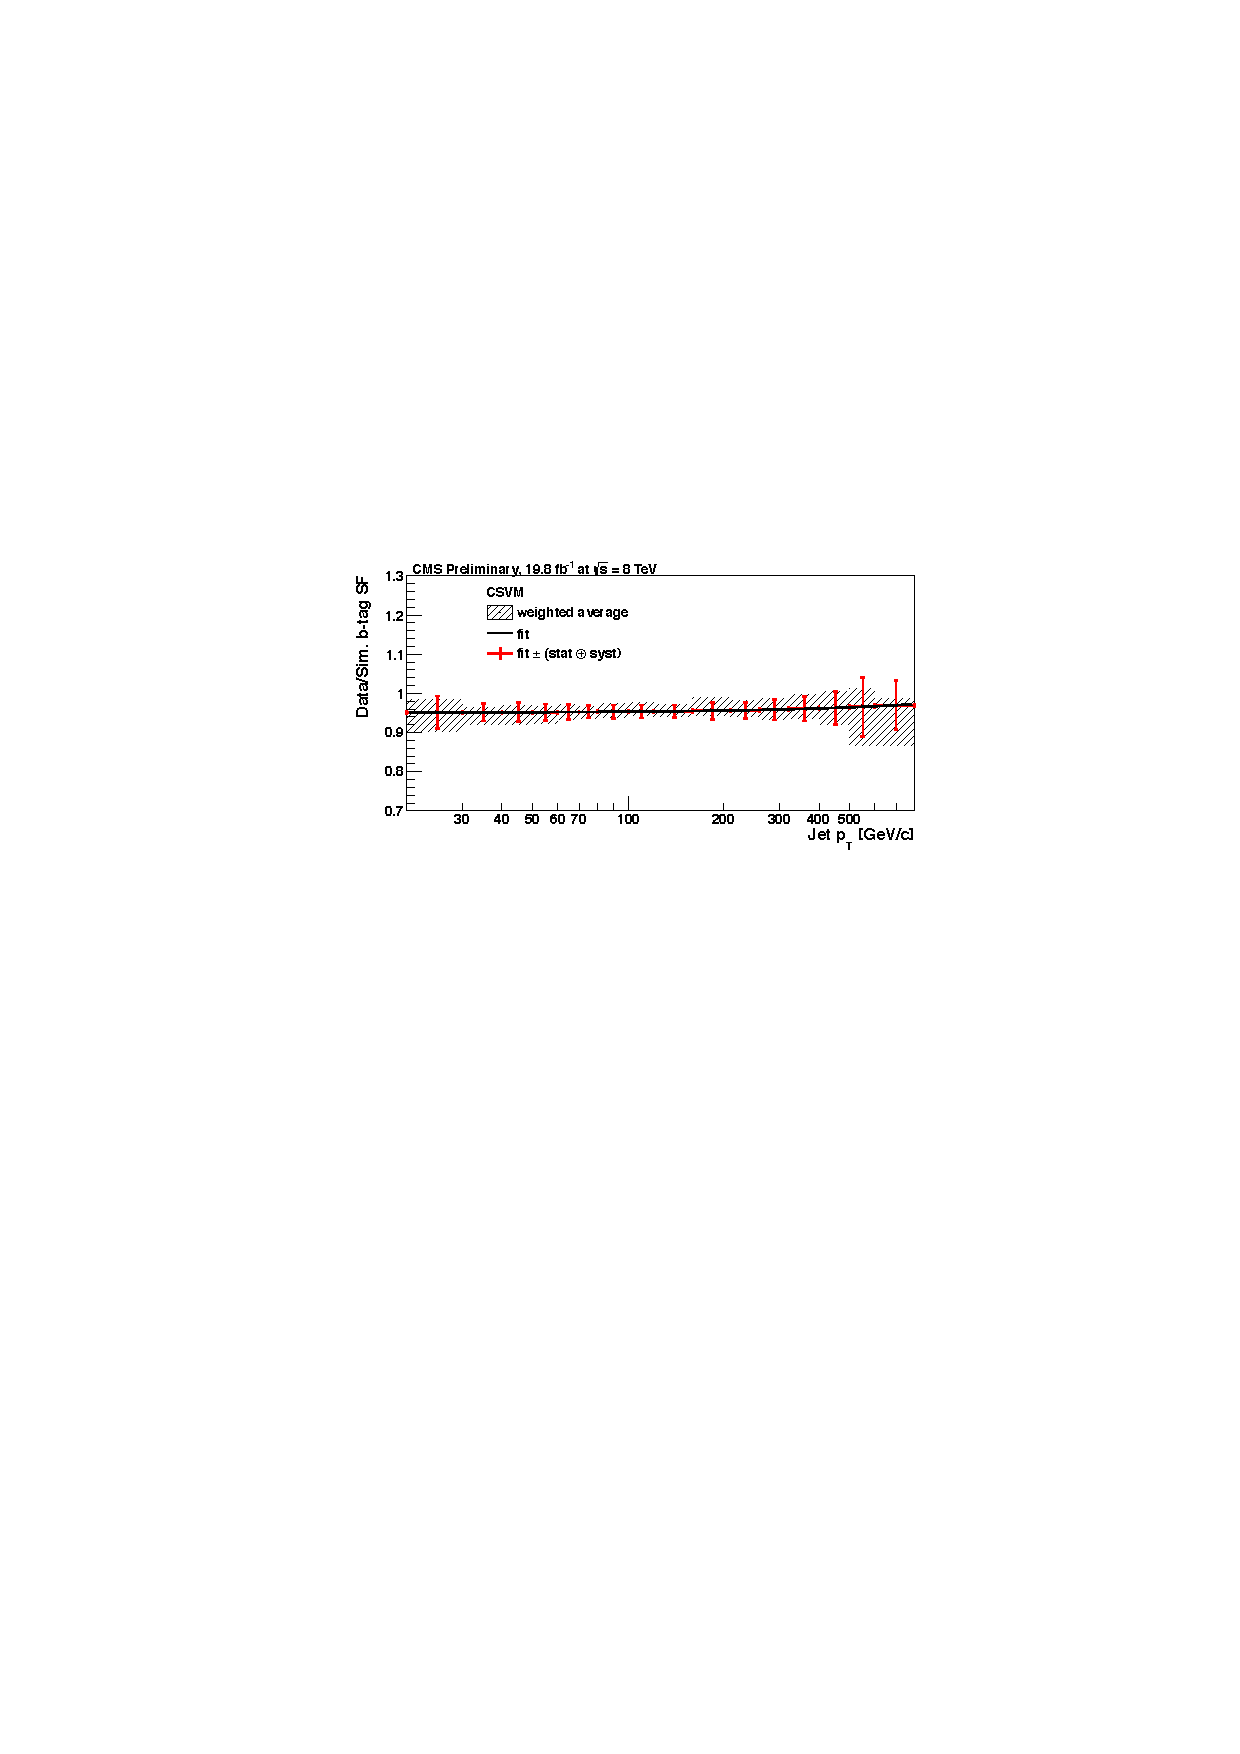
\includegraphics[width=0.6\textwidth]{Figures/b-tagSF.pdf}
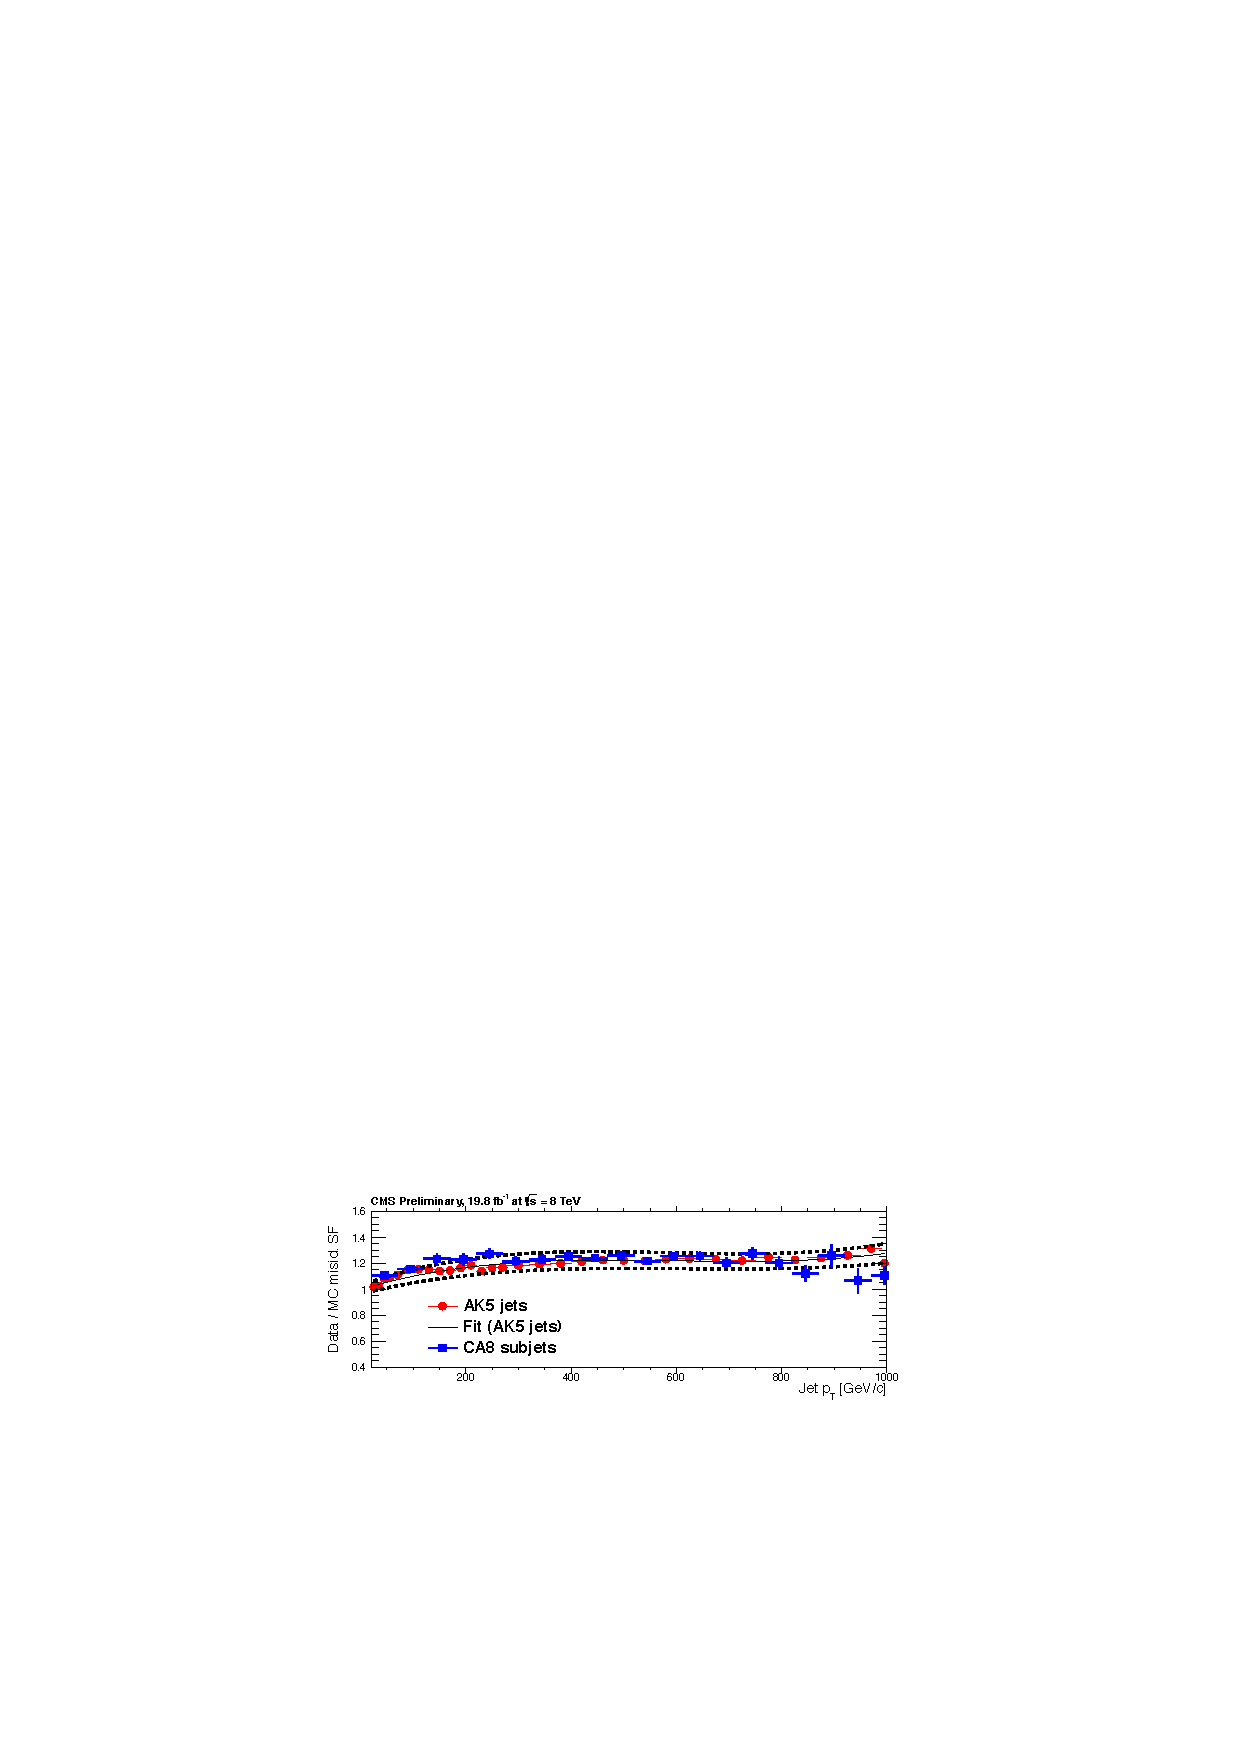
\includegraphics[width=0.6\textwidth]{Figures/miss-tag.pdf}
\label{fig:bSF}
\caption{B-tagging scale factora and misstag scale factors}
\end{figure}

 